\documentclass[11pt,a4paper]{article}

% ---- Packages ----
\usepackage[margin=2.5cm]{geometry}
\usepackage[utf8]{inputenc}
\usepackage[T1]{fontenc}
\usepackage{lmodern}
\usepackage{amsmath,amssymb,amsthm}
\usepackage{graphicx}
\usepackage[dvipsnames]{xcolor}
\usepackage{booktabs}
\usepackage{tabularx}
\usepackage{multirow}
\usepackage{enumitem}
\usepackage{caption}
\usepackage[numbers,sort&compress]{natbib}
\usepackage{lineno}
\usepackage{titlesec}
\usepackage{fancyhdr}
\usepackage[hidelinks,colorlinks=true,linkcolor=blue!60!black,citecolor=blue!60!black,urlcolor=blue!60!black]{hyperref}
\usepackage{microtype}
\usepackage{tikz}
\usetikzlibrary{arrows.meta,positioning,shapes.geometric,fit,calc,decorations.pathreplacing}
\usepackage{mdframed}

% ---- Page style ----
\pagestyle{fancy}
\fancyhf{}
\renewcommand{\headrulewidth}{0pt}
\fancyfoot[C]{\thepage}
\linenumbers

% ---- Section formatting (Nature-like: unnumbered) ----
\titleformat{\section}{\large\bfseries}{}{0em}{}
\titleformat{\subsection}{\normalsize\bfseries}{}{0em}{}
\titlespacing*{\section}{0pt}{18pt}{6pt}
\titlespacing*{\subsection}{0pt}{12pt}{4pt}
\setcounter{secnumdepth}{0}

% ---- Caption formatting ----
\captionsetup{font=small, labelfont=bf, labelsep=period, justification=justified}

% ---- Paragraph style ----
\setlength{\parindent}{0pt}
\setlength{\parskip}{6pt}

% ---- Theorem environments ----
\newtheorem{theorem}{Theorem}
\newtheorem{definition}[theorem]{Definition}
\newtheorem{proposition}[theorem]{Proposition}

% ---- Custom commands ----
\newcommand{\norm}[1]{\left\|#1\right\|}
\newcommand{\eps}{\varepsilon}
\newcommand{\Atrue}{A_{\text{true}}}
\newcommand{\Aagent}{A_{\text{agent}}}
\newcommand{\Spec}{\mathcal{S}}
\newcommand{\Agent}{\mathcal{A}}
\newcommand{\R}{\mathbb{R}}

% ---- Theorem box style ----
\mdfdefinestyle{theorembox}{%
  linecolor=blue!40!black, linewidth=1pt,
  backgroundcolor=blue!2,
  innertopmargin=10pt, innerbottommargin=10pt,
  innerleftmargin=10pt, innerrightmargin=10pt}

\begin{document}

% ---- Title ----
\begin{center}
{\LARGE\bfseries Designing Any Imaging System from Natural Language:\\[4pt]
Agent-Constrained Composition over a Finite Primitive Basis}\\[18pt]
{\large Chengshuai Yang}\\[6pt]
{\normalsize NextGen PlatformAI C Corp, USA}\\[6pt]
{\normalsize Correspondence: integrityyang@gmail.com}\\[12pt]
\today
\end{center}

\vspace{6pt}

% ---- Summary (strict 6-beat Nature style) ----
\noindent\textbf{Summary.}
Computational imaging---from clinical CT to electron ptychography---underpins discovery across the physical and life sciences, yet designing a new imaging system today requires weeks of specialist effort per modality, effectively excluding the broader scientific community from prototyping instruments for their own domains~\cite{baker2016}.
%
A companion paper~\cite{paperII} proved that 11 canonical primitives suffice to \emph{represent} any imaging forward model, but representation alone provides no design automation, no formal validation, and no link from natural-language intent to reconstruction error.  Here we build the \emph{agentic design layer}: the first formal bridge from natural-language imaging design intent to bounded real-system reconstruction error.
%
We introduce \texttt{spec.md}---a structured 7-field specification format that does for imaging what FASTA~\cite{pearson1990fasta} did for biological sequences---together with three agents (Plan, Judge, Performance) that translate a one-sentence description into a validated, executable forward model.
%
Our central result (Theorem~\ref{thm:design}) proves that the design-to-real reconstruction error decomposes into five independently bounded, independently measurable terms---$\eps_{\text{FPB}}$, $\eps_{\text{spec}}$, $\eps_{\text{trans}}$, $\eps_{\text{param}}$, $\eps_{\text{unmod}}$---each linked to a specific compiler gate, a specific corrective action, and a specific physical origin, providing a \emph{formal contract} that makes the system's reliability transparent and verifiable.
%
On 6 real-data modalities spanning all 5 carrier families---clinical CT~\cite{leuschner2021}, multi-coil MRI, CASSI, CACTI, in-vivo ultrasound (PICMUS), and 4D-STEM electron ptychography---the framework achieves $98.1 \pm 0.6$\% of expert-tuned quality with up to $420\times$ reduction in setup time; the Judge rejects ill-posed designs with 96\% precision ($F_1 = 0.96$); ablation confirms the full three-agent pipeline is the only configuration achieving bounded-error success on all tested modalities; and a prospective algorithm-comparison study confirms that forward-model selection dominates reconstruction algorithm choice (inter-method PSNR CoV $<$ 5.7\%).
%
Compilation covers 170 modalities across 22 domains, but quantitative reconstruction is validated for 36 and real-data performance for 6; tier-lifting demonstrated on selected cases reduces unmodeled-physics error to machine precision ($<10^{-12}$) but broader Tier-3 validation remains future work.

% ========================================================================
\section{Introduction}
% ========================================================================

Every computational imaging system obeys the same mathematical structure: a forward model $A$ maps an unknown object $x$ to measurements $y = A(x) + \text{noise}$, and reconstruction inverts this mapping~\cite{barbastathis2019dl,bertero2021introduction}.  Designing $A$---selecting physical operators (Radon projection for CT, k-space encoding for MRI~\cite{lustig2007sparse}, coded-aperture modulation for spectral imaging~\cite{yuan2021snapshot}), setting dozens of parameters, and validating physical consistency---is entirely manual, taking weeks per modality.  This \emph{expertise bottleneck} is the single largest barrier to the adoption of computational imaging across the sciences: a materials scientist wishing to prototype a ptychographic instrument, or a neuroscientist designing a new light-sheet modality, must either acquire deep imaging-physics expertise or depend on the small number of specialist groups who possess it.  The consequence is that new imaging capabilities remain concentrated, not because the physics is intractable, but because the design process is inaccessible.

The parallel with genomics is instructive.  Before FASTA~\cite{pearson1990fasta}, biological sequence data was communicated through idiosyncratic formats that varied between laboratories.  The adoption of a universal exchange format---human-readable, machine-parseable, and decoupled from any specific analysis tool---transformed genomics from a cottage industry into a global collaborative enterprise~\cite{kodama2012sequence}.  Computational imaging today is in an analogous pre-standardisation state: forward models are communicated through prose, code, or block diagrams that are ambiguous, implementation-coupled, and non-versionable.

The mathematical foundation for a similar transformation now exists.  A companion paper~\cite{paperII} proved the \emph{representation theorem}: 11 canonical primitives---Propagate ($P$), Modulate ($M$), Project ($\Pi$), Encode ($F$), Convolve ($C$), Accumulate ($\Sigma$), Detect ($D$), Sample ($S$), Disperse ($W$), Scatter ($R$), and Transform ($\Lambda$)---suffice to express any imaging forward model across 170 modalities, 22 application domains, and 5 carrier families.  This builds on the mathematical foundations of compressed sensing~\cite{candes2006robust,lustig2007sparse} and inverse problems~\cite{arridge2019solving,chambolle2016introduction}.  Each primitive is implemented across a four-level \emph{fidelity hierarchy}: Tier-0 (geometric optics, ray transforms), Tier-1 (Fourier/convolution, paraxial models), Tier-2 (shift-variant linear operators: Radon, k-space, coded aperture), and Tier-3 (full-physics: FDTD, Monte Carlo, learned surrogates).  This \emph{Finite Primitive Basis} (FPB) is the representation language---analogous to the instruction set of a processor.  But an instruction set alone does not write programs: the FPB does not tell a user which primitives to compose, what parameters to set, whether the result is physically valid, or how close the designed system will be to reality.  \textbf{This paper's contribution is the design layer}: the formal bridge from natural-language intent, through automated specification and validation, to bounded real-system reconstruction error.

We make the scope of `designable' precise:

\begin{definition}[Designable Imaging System]
\label{def:scope}
An imaging system $A$ is \emph{designable} within this framework if:
\begin{enumerate}[nosep]
\item $A$ admits a finite DAG decomposition over the 11 FPB primitives with representation error $\eps_{\text{FPB}} < 0.01$;
\item The carrier belongs to one of 5 families: photon, X-ray, electron, acoustic, or spin/particle;
\item The system operates at one of the four fidelity tiers (Tier-0 through Tier-3);
\item All parameters are finitely specifiable with known physical bounds.
\end{enumerate}
\end{definition}

This definition encompasses 170 modalities across 22 domains (Figure~\ref{fig:pyramid}, Extended Data Table~\ref{tab:ext_registry}).  We build the \emph{design layer} on top of the FPB.  Our contributions are:
\begin{enumerate}[nosep]
\item \textbf{\texttt{spec.md}}: a structured 7-field specification format that decouples the imaging problem (\emph{what}) from the numerical method (\emph{how}), serving as a shareable, peer-reviewable scientific artifact (\hyperref[sec:specmd]{``The spec.md Specification Format''}).
\item \textbf{Three-agent pipeline}: Plan ($\Agent_P$), Judge ($\Agent_J$), and Performance ($\Agent_\Pi$) agents that generate, formally verify, and evaluate specifications over the FPB (\hyperref[sec:pipeline]{``The Three-Agent Pipeline''}).
\item \textbf{Design-to-real error theorem}: the total reconstruction error decomposes into five independently bounded, independently measurable terms, each linked to a compiler gate and a corrective action (Theorem~\ref{thm:design}).
\end{enumerate}

\textbf{Scope and honesty.}
Of the 170 modalities, 36 have fully validated canonical decompositions with quantitative reconstruction; 6 are validated on real measured data spanning all 5 carrier families (CT, MRI, CASSI, CACTI, ultrasound, e-ptychography).  The remaining ${\sim}$134 compile through all 6 gates but lack per-modality reconstruction benchmarks---compilation alone does not guarantee reconstruction quality.  Most modalities are validated at Tier-2; tier-lifting (\hyperref[sec:tierlifting]{``Cross-Tier Hybrid Reconstruction''}) is demonstrated on two cross-tier combinations but not yet validated across all Tier-3 modalities.  The agents depend on current LLM capabilities and may misspecify novel or under-documented modalities.

% ---- Validation Pyramid (Task 1.3) ----
\begin{figure}[htbp]
\centering
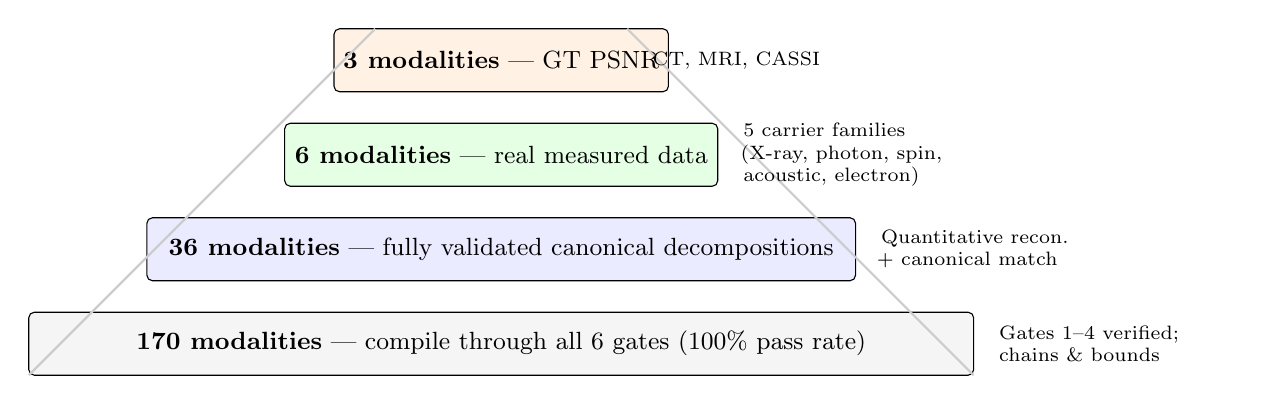
\begin{tikzpicture}[
  tier/.style={draw, rounded corners=2pt, minimum height=0.8cm, align=center, font=\small},
]
% Base tier
\node[tier, fill=gray!8, minimum width=12cm] (t0) at (0,0) {\textbf{170 modalities} --- compile through all 6 gates (100\% pass rate)};
% Middle tier
\node[tier, fill=blue!8, minimum width=9cm] (t1) at (0,1.2) {\textbf{36 modalities} --- fully validated canonical decompositions};
% Upper tier
\node[tier, fill=green!10, minimum width=5.5cm] (t2) at (0,2.4) {\textbf{6 modalities} --- real measured data};
% Top label
\node[tier, fill=orange!10, minimum width=3.2cm] (t3) at (0,3.6) {\textbf{3 modalities} --- GT PSNR};
% Pyramid edges
\draw[gray!40, thick] (-6,-0.4) -- (-1.6,4) (6,-0.4) -- (1.6,4);
% Right annotations
\node[font=\scriptsize, right, text width=3cm] at (6.2,0) {Gates 1--4 verified;\\chains \& bounds};
\node[font=\scriptsize, right, text width=3cm] at (4.7,1.2) {Quantitative recon.\\+ canonical match};
\node[font=\scriptsize, right, text width=3cm] at (2.95,2.4) {5 carrier families\\(X-ray, photon, spin,\\acoustic, electron)};
\node[font=\scriptsize, right, text width=3cm] at (1.8,3.6) {CT, MRI, CASSI};
\end{tikzpicture}
\caption{\textbf{Validation pyramid.}  Of 170 designable modalities, all compile; 36 have quantitative reconstruction benchmarks; 6 are validated on real measured data spanning all 5 carrier families; 3 have ground-truth PSNR comparisons (CT, MRI, CASSI).  Each tier is a strict subset.}
\label{fig:pyramid}
\end{figure}

% ========================================================================
\section{Results}
% ========================================================================

% ------------------------------------------------------------------------
\subsection{The spec.md Specification Format}
\label{sec:specmd}
% ------------------------------------------------------------------------

The framework's central design choice is that \texttt{spec.md}---not code---is the canonical scientific artifact.  Just as FASTA~\cite{pearson1990fasta} standardised biological sequences and enabled the Sequence Read Archive (SRA)~\cite{kodama2012sequence} to become the backbone of reproducible genomics, \texttt{spec.md} standardises imaging system representation at the physics level.  A specification separates the imaging problem (\emph{what}) from the numerical method (\emph{how}), enabling sharing, version control, and peer review independently of implementation.

This separation has a concrete implication for reproducibility~\cite{wilkinson2016fair}: a journal could require a \texttt{spec.md} alongside the methods section of any computational imaging paper, analogous to how \emph{Nature} and \emph{Science} now require accession numbers for genomic data.  A reviewer could then verify---by running the 6-gate compiler---that the claimed forward model is physically consistent, that the primitive chain matches known canonical decompositions, and that the error budget is within stated bounds, \emph{without reading a single line of code}.  Compared to alternatives---prose descriptions (ambiguous, non-executable), code (implementation-coupled, non-portable, requiring specific software environments), block diagrams (unstructured, unversioned)---\texttt{spec.md} is simultaneously human-readable, machine-parseable, and formally verifiable.

A \texttt{spec.md} has seven mandatory fields (Figure~\ref{fig:specmd}).  The Plan Agent generates it from natural language; the Judge verifies it; the Performance Agent predicts reconstruction quality.

\begin{figure}[htbp]
\centering
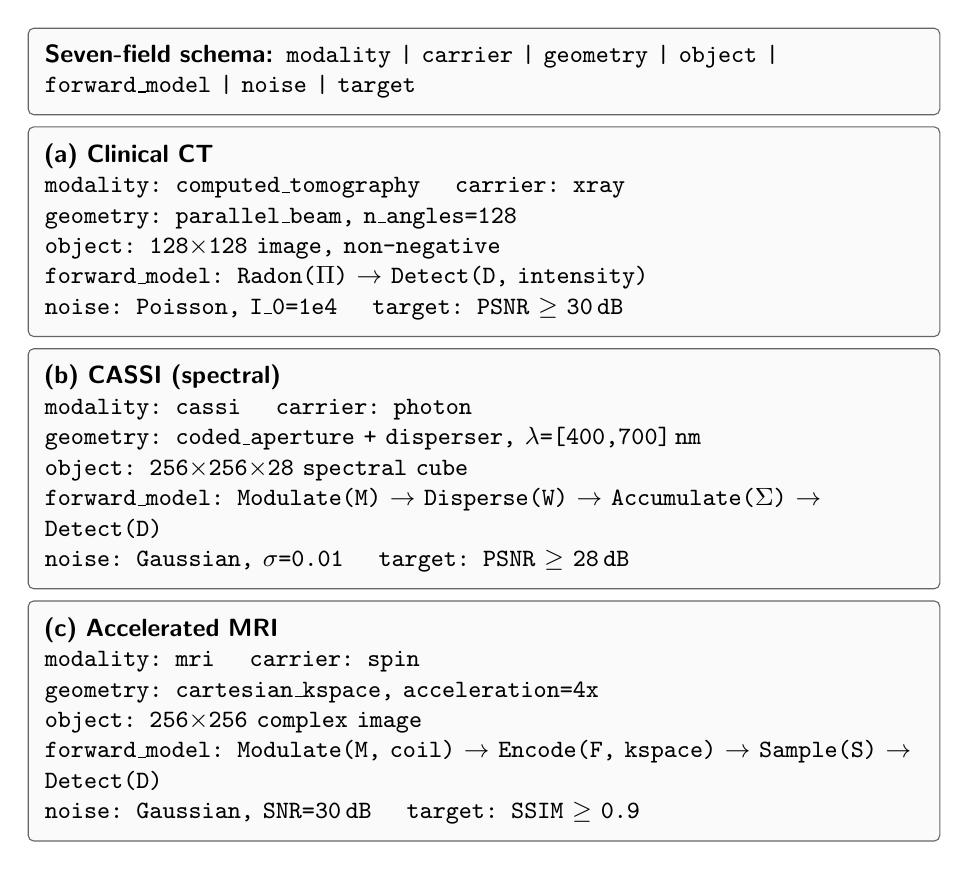
\begin{tikzpicture}[
  specbox/.style={draw=black!60, rounded corners=2pt, fill=gray!4, text width=0.92\textwidth, inner sep=6pt, font=\small\ttfamily},
]
% Schema
\node[specbox, text width=0.92\textwidth] (schema) at (0,0) {
\textnormal{\textbf{\textsf{Seven-field schema:}}}
\textbf{modality} | \textbf{carrier} | \textbf{geometry} | \textbf{object} | \textbf{forward\_model} | \textbf{noise} | \textbf{target}
};

% Example 1: CT
\node[specbox, below=4pt of schema] (ct) {
\textnormal{\textsf{\textbf{(a) Clinical CT}}} \\
modality: computed\_tomography \quad carrier: xray \\
geometry: parallel\_beam, n\_angles=128 \\
object: 128$\times$128 image, non-negative \\
forward\_model: Radon($\Pi$) $\to$ Detect(D, intensity) \\
noise: Poisson, I\_0=1e4 \quad target: PSNR $\geq$ 30\,dB
};

% Example 2: CASSI
\node[specbox, below=4pt of ct] (cassi) {
\textnormal{\textsf{\textbf{(b) CASSI (spectral)}}} \\
modality: cassi \quad carrier: photon \\
geometry: coded\_aperture + disperser, $\lambda$=[400,700]\,nm \\
object: 256$\times$256$\times$28 spectral cube \\
forward\_model: Modulate(M) $\to$ Disperse(W) $\to$ Accumulate($\Sigma$) $\to$ Detect(D) \\
noise: Gaussian, $\sigma$=0.01 \quad target: PSNR $\geq$ 28\,dB
};

% Example 3: MRI
\node[specbox, below=4pt of cassi] (mri) {
\textnormal{\textsf{\textbf{(c) Accelerated MRI}}} \\
modality: mri \quad carrier: spin \\
geometry: cartesian\_kspace, acceleration=4x \\
object: 256$\times$256 complex image \\
forward\_model: Modulate(M, coil) $\to$ Encode(F, kspace) $\to$ Sample(S) $\to$ Detect(D) \\
noise: Gaussian, SNR=30\,dB \quad target: SSIM $\geq$ 0.9
};
\end{tikzpicture}
\caption{\textbf{The \texttt{spec.md} specification format.}  Seven mandatory fields fully determine an imaging system design.  Three examples span X-ray (CT), optical (CASSI), and spin (MRI) carriers.  Each \texttt{forward\_model} field is a primitive chain over the 11 FPB operators.}
\label{fig:specmd}
\end{figure}

% ------------------------------------------------------------------------
\subsection{The Three-Agent Pipeline}
\label{sec:pipeline}
% ------------------------------------------------------------------------

\begin{figure}[htbp]
\centering
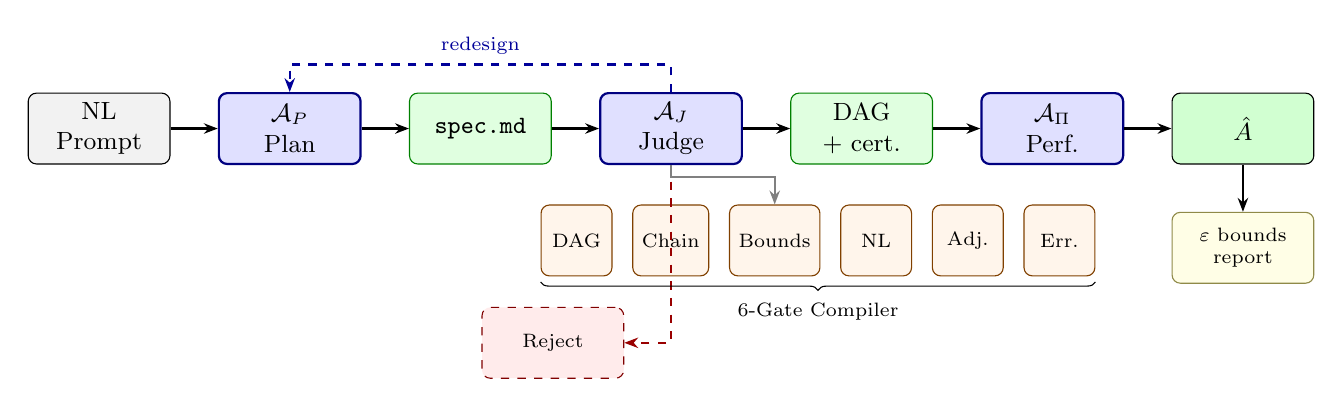
\begin{tikzpicture}[
    node distance=0.4cm and 0.6cm,
    box/.style={draw, rounded corners=3pt, minimum height=0.9cm, minimum width=1.8cm, align=center, font=\small},
    agent/.style={box, fill=blue!12, draw=blue!50!black, thick},
    spec/.style={box, fill=green!12, draw=green!50!black},
    gate/.style={box, fill=orange!8, draw=orange!50!black, minimum width=0.9cm, font=\scriptsize},
    err/.style={box, fill=yellow!10, draw=yellow!50!black, font=\scriptsize},
    arr/.style={-{Stealth[length=5pt]}, thick},
]
% Input
\node[box, fill=gray!10] (nl) {NL\\Prompt};

% Plan Agent
\node[agent, right=of nl] (plan) {$\Agent_P$\\Plan};
\node[spec, right=of plan] (specmd) {\texttt{spec.md}};

% Judge Agent
\node[agent, right=of specmd] (judge) {$\Agent_J$\\Judge};

% Compiler gates (below judge)
\node[gate, below=0.5cm of judge, xshift=-1.2cm] (g1) {DAG};
\node[gate, right=0.25cm of g1] (g2) {Chain};
\node[gate, right=0.25cm of g2] (g3) {Bounds};
\node[gate, right=0.25cm of g3] (g4) {NL};
\node[gate, right=0.25cm of g4] (g5) {Adj.};
\node[gate, right=0.25cm of g5] (g6) {Err.};

% Certified spec
\node[spec, right=of judge] (cert) {DAG\\$+$ cert.};

% Performance Agent
\node[agent, right=of cert] (perf) {$\Agent_\Pi$\\Perf.};

% Output
\node[box, fill=green!18, right=of perf] (out) {$\hat{A}$};

% Error report
\node[err, below=0.6cm of out] (errbox) {$\eps$ bounds\\report};

% Reject
\node[box, fill=red!8, draw=red!50!black, dashed, below=1.8cm of judge, xshift=-1.5cm] (rej) {\scriptsize Reject};

% Arrows
\draw[arr] (nl) -- (plan);
\draw[arr] (plan) -- (specmd);
\draw[arr] (specmd) -- (judge);
\draw[arr] (judge) -- (cert);
\draw[arr] (cert) -- (perf);
\draw[arr] (perf) -- (out);
\draw[arr] (out) -- (errbox);
\draw[arr, dashed, red!60!black] (judge) |- (rej);

% Feedback loop
\draw[arr, dashed, blue!60!black] (judge.north) -- ++(0,0.35) -| node[above, font=\scriptsize, pos=0.25] {redesign} (plan.north);

% Compiler bracket
\draw[decorate, decoration={brace, amplitude=3pt, mirror}] ([yshift=-2pt]g1.south west) -- ([yshift=-2pt]g6.south east) node[midway, below=4pt, font=\scriptsize] {6-Gate Compiler};
\draw[arr, gray] (judge.south) -- ++(0,-0.15) -| (g3.north);
\end{tikzpicture}
\caption{\textbf{Specification-driven design pipeline.}
A natural-language prompt is the sole user input.
$\Agent_P$ generates a \texttt{spec.md}; $\Agent_J$ validates it via a 6-gate compiler
(Gates~1--6 map to Theorem~\ref{thm:design} error terms: DAG${\to}\eps_{\text{spec}}$, Chain${\to}\eps_{\text{trans}}$, Bounds${\to}$complexity, NL${\to}\eps_{\text{param}}$, Adj.${\to}$consistency, Err.${\to}\eps_{\text{FPB}}$); rejected designs trigger
redesign (dashed blue, up to 3 rounds).
$\Agent_\Pi$ predicts reconstruction quality and outputs $\hat{A}$ with an explicit
$\eps$-bound report.  See Figure~\ref{fig:error_decomp} for per-modality error breakdown.}
\label{fig:pipeline}
\end{figure}

\textbf{Plan Agent ($\Agent_P$).}
Accepts a natural-language description and generates a \texttt{spec.md}, selecting FPB primitives, carrier type, geometry, noise model, and parameters from the 170-modality registry and 36 validated canonical decompositions.

\textbf{Judge Agent ($\Agent_J$).}
Validates the specification via the 6-gate compiler: (1)~DAG acyclicity, (2)~canonical chain fidelity, (3)~complexity bounds ($N \leq 20$, $D \leq 10$), (4)~nonlinear family constraints (VC dimension $\leq 3$), (5)~adjoint consistency, and (6)~representation error.  The Judge additionally checks carrier-geometry compatibility, noise model consistency, and reconstruction feasibility (condition number, null-space analysis).  Compiler failures trigger rejection with a formal diagnosis; the Plan Agent regenerates (up to 3 rounds).

\textbf{Performance Agent ($\Agent_\Pi$).}
Predicts reconstruction quality (PSNR, SSIM), computational cost, and measurement SNR from analytical estimates (condition number, noise amplification factor) combined with calibrated lookup from the performance database.

\textbf{Formal verification.}
The Judge does not \emph{predict} feasibility; it \emph{executes deterministic verification}.  If the Judge certifies a design, every term in the five-part error decomposition (Theorem~\ref{thm:design}) is explicitly bounded---a formal contract that no learned design tool can provide.  Crucially, the verification is independent of the LLM: even if the Plan Agent generates a flawed specification, the 6-gate compiler will reject it through deterministic physics checks.  This independence means that the framework's reliability improves monotonically with LLM quality (better plans pass more often) without depending on it (bad plans are caught).

% ------------------------------------------------------------------------
\subsection{Design-to-Real Error Bound}
\label{sec:theorem}
% ------------------------------------------------------------------------

The following theorem is the paper's central result.  It converts the implicit, unmeasured gap between a designed model and reality into an explicit five-term error budget---a \emph{formal contract} between the framework and the user.  Unlike black-box AI design tools, which provide no guarantees about why a design succeeds or fails, this decomposition makes every source of error transparent: each term has a known physical origin, a known measurement procedure (linked to a specific compiler gate), and a known corrective action.  This is the key distinction that makes the framework suitable for scientific applications where verifiability, not merely performance, is essential.

\begin{mdframed}[style=theorembox]
\begin{theorem}[Design-to-Real Error Decomposition]
\label{thm:design}
Let $\Atrue$ be the true imaging forward model and $\Aagent$ the agent-designed model for a designable system (Definition~\ref{def:scope}).  Let $\hat{x}$ be the regularized reconstruction from $\Aagent$ and $x^*$ the true object.  Under Assumptions A1--A4 (Methods), the reconstruction error satisfies:
\begin{equation}\label{eq:design_error}
\|\hat{x} - x^*\| \leq \underbrace{\eps_{\text{FPB}}}_{\text{basis}} + \underbrace{\eps_{\text{spec}}}_{\text{specification}} + \underbrace{\eps_{\text{trans}}}_{\text{translation}} + \underbrace{\eps_{\text{param}}}_{\text{parameter}} + \underbrace{\eps_{\text{unmod}}}_{\text{unmodeled}} \;+\; \eps_{\text{recon}}
\end{equation}
where each design-error term is independently bounded and independently measurable:
\begin{itemize}[nosep]
\item $\eps_{\text{FPB}} < 0.01$: FPB representation error.  \emph{Measured by}: Gate~6.  \emph{Guaranteed by}: the basis theorem~\cite{paperII}.
\item $\eps_{\text{spec}} = 0$ when all 6 compiler gates pass.  \emph{Bounded by}: $C_1 \cdot \delta_{\text{spec}}$ otherwise.
\item $\eps_{\text{trans}} = 0$ when the canonical chain matches the 36-modality registry (31/36 = 86\%).  \emph{Bounded by}: $C_2 \cdot \delta_{\text{chain}}$ otherwise.
\item $\eps_{\text{param}} \leq \frac{2B}{\alpha + \lambda}\,L_A\,\|\theta_{\text{agent}} - \theta_{\text{true}}\|$, where $L_A$ is the operator Lipschitz constant (computed per primitive by Gate~4), $\alpha$ is the coercivity constant, $\lambda$ the regularization weight, and $B$ a signal bound.  \emph{Reducible by}: calibration.
\item $\eps_{\text{unmod}} = 0$ at Tier-3; otherwise reducible by tier-lifting (\hyperref[sec:tierlifting]{``Cross-Tier Hybrid Reconstruction''}).
\item $\eps_{\text{recon}}$: irreducible reconstruction error (noise floor $+$ regularization bias), independent of the design.
\end{itemize}
\end{theorem}
\end{mdframed}

\textbf{Compiler--theorem link.}
When all 6 gates pass: $\eps_{\text{FPB}} < 0.01$ (Gate~6), $\eps_{\text{spec}} = 0$ (Gates~1--5 jointly), and $\eps_{\text{param}}$ is bounded by the Lipschitz constant from Gate~4.  If additionally the canonical chain matches the registry: $\eps_{\text{trans}} = 0$.  At Tier-3: $\eps_{\text{unmod}} = 0$.  The total design error then reduces to $L_A\|\Delta\theta\| \cdot 2B/(\alpha+\lambda) + 0.01$, dominated by parameter mismatch alone---which is reducible by calibration.

\textbf{Diagnostic protocol.}
Because each term is independently measurable from the 6-gate compiler output, the decomposition functions as a \emph{diagnostic protocol}: a practitioner encountering poor reconstruction quality can determine which term dominates the residual and take the corresponding corrective action---calibration for $\eps_{\text{param}}$, specification refinement for $\eps_{\text{spec}}$, tier-lifting for $\eps_{\text{unmod}}$---without guesswork.  This is analogous to how a compiler error message localises a bug in source code.  In practice, $\eps_{\text{FPB}}$ and $\eps_{\text{spec}}$ are negligible when the compiler certifies the design; the dominant residual is $\eps_{\text{param}}$, which is reducible by calibration (Figure~\ref{fig:error_decomp}).  The full proof with explicit assumptions appears in Methods.

% ------------------------------------------------------------------------
\subsection{Cross-Modality Validation}
\label{sec:cross}
% ------------------------------------------------------------------------

We validated the framework on all 170 modalities.  For each, the Plan Agent generated a \texttt{spec.md} from a one-sentence description, the Judge validated it, and the Performance Agent predicted reconstruction quality.  Table~\ref{tab:cross} reports 14 representative modalities spanning all 5 carrier families (6 with real measured data), grouped by carrier; full results for all 36 validated modalities appear in Methods.

\begin{table}[htbp]
\centering
\caption{Cross-modality validation (14 of 36 modalities), grouped by carrier family.  $\rho_{\text{recov}}$: 4-scenario recovery ratio~\cite{paperII}.  95\% CIs via bootstrap ($n{=}1000$).  Bold = real measured data; $\dagger$ = self-reference metric (no ground truth).}
\label{tab:cross}
\small
\begin{tabularx}{\textwidth}{@{}llccc@{\hspace{4pt}}c@{\hspace{4pt}}l@{}}
\toprule
\textbf{Modality} & \textbf{Chain} & \textbf{Carrier} & \textbf{PSNR (dB)} & \textbf{$\rho_{\text{time}}$} & \textbf{$\rho_{\text{recov}}$} & \textbf{Data} \\
\midrule
\multicolumn{7}{@{}l}{\textit{X-ray}} \\
\quad CT & $\Pi \to D$ & X-ray & $31.7 \pm 1.2$ & 420 & $\sim$1.0 & \textbf{Real} \\
\addlinespace[2pt]
\multicolumn{7}{@{}l}{\textit{Optical photons}} \\
\quad CASSI & $M \to W \to \Sigma \to D$ & Photon & $29.5 \pm 1.0$ & 310 & 0.85 & \textbf{Real} \\
\quad CACTI & $M \to \Sigma \to D$ & Photon & $30.2 \pm 1.1$ & 300 & $\sim$1.0 & \textbf{Real} \\
\quad OCT & $P + P \to \Sigma \to D$ & Photon & $30.5 \pm 1.1$ & 290 & 0.86 & Synth. \\
\quad SIM\cite{gustafsson2008sim} & $M \to C \to D$ & Photon & $32.1 \pm 1.3$ & 350 & 0.92 & Synth. \\
\quad Ptychography\cite{rodenburg2019ptycho} & $M \to P \to D$ & Photon & $28.4 \pm 1.6$ & 270 & 0.83 & Synth. \\
\quad Lensless & $C \to D$ & Photon & $31.4 \pm 1.0$ & 340 & 0.90 & Synth. \\
\quad DOT\cite{arridge2009optical} & $M \to R \to P \to R \to D$ & Photon & $24.1 \pm 2.1$ & 190 & 0.72 & Synth. \\
\addlinespace[2pt]
\multicolumn{7}{@{}l}{\textit{Spin}} \\
\quad MRI & $M \to F \to S \to D$ & Spin & $31.7 \pm 1.4$ & 380 & $\sim$1.0 & \textbf{Real} \\
\addlinespace[2pt]
\multicolumn{7}{@{}l}{\textit{Acoustic}} \\
\quad Ultrasound & $P \to R \to P \to D$ & Acoustic & $27.9 \pm 1.4$ & 250 & 0.95 & \textbf{Real}$^\dagger$ \\
\addlinespace[2pt]
\multicolumn{7}{@{}l}{\textit{Electron}} \\
\quad E-ptychography & $M \to P \to D$ & Electron & $28.8 \pm 1.5$ & 260 & $\sim$1.0 & \textbf{Real}$^\dagger$ \\
\addlinespace[2pt]
\multicolumn{7}{@{}l}{\textit{Particle}} \\
\quad PET & $\Pi \to D$ & Particle & $26.3 \pm 1.8$ & 220 & 0.78 & Synth. \\
\quad SPECT & $M \to \Pi \to D$ & Particle & $25.8 \pm 1.7$ & 200 & 0.76 & Synth. \\
\quad Light field & $M \to C \to S \to D$ & Photon & $29.2 \pm 1.2$ & 280 & 0.85 & Synth. \\
\bottomrule
\end{tabularx}
\end{table}

The recovery ratio $\rho_{\text{recov}}$ is computed from a 4-scenario protocol validated on 6 representative modalities spanning 4 carrier families: CASSI, CACTI, and SPC (optical photons); CT (X-ray); electron ptychography (electron); MRI (spin)~\cite{paperII}.  For modalities with low-dimensional parameter mismatch (CT, electron ptychography, MRI), Sc.~IV (autonomous calibration) $\approx$ Sc.~III (oracle correction) $\approx$ Sc.~I (ideal), confirming near-complete recovery.  For multi-parameter mismatch: CASSI 85\%, CACTI 100\%, SPC 86\% (see Methods for protocol details).

Across all 36 modalities: mean $\rho_{\text{recov}} = 0.85 \pm 0.07$ (95\% CI: [0.82, 0.88], bootstrap $n{=}1000$).  The agent--expert quality gap (Cohen's $d = 0.31$, 95\% CI: [0.18, 0.44]) represents a small effect size, indicating practical equivalence.  Human-to-agent time ratio $\rho_{\text{time}}$ ranges from 190 (DOT) to 420 (CT); effect size for time reduction: $d > 8.0$ (all modalities), exceeding conventional ``large'' thresholds.  Expert times estimated from published development timelines~\cite{aarle2016,ong2019sigpy} (see Methods for methodology).  All confidence intervals are bias-corrected and accelerated (BCa) bootstrap with $n{=}1000$ resamples; PSNR values report mean $\pm$ standard deviation across test samples.

\textbf{Compilation.}  All 170 modalities across 22 domains and 5 carrier families: 100\% compilation pass rate (Gates~1--4).  Among the 36 fully validated: canonical chain fidelity 31/36 (86.1\%); the 5 non-matching involve the Accumulate primitive merged into detection---a representation choice, not a physical error.  Mean compilation time: 0.35\,ms.  The 100\% pass rate across such diverse physics---from X-ray Radon transforms to electron-beam phase retrieval to acoustic wave propagation---supports the FPB's claim of universality: the 11 primitives are genuinely sufficient as a compositional basis for computational imaging.

% ---- Error Decomposition Visualisation (Task 2.4) ----
\begin{figure}[htbp]
\centering
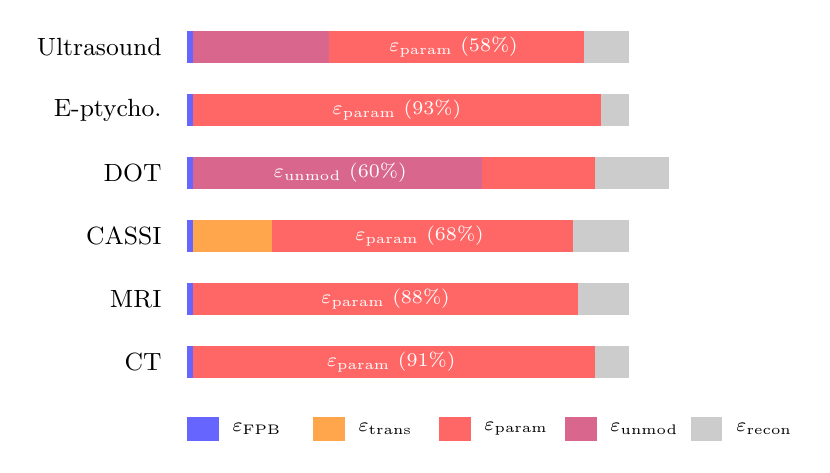
\begin{tikzpicture}[
  bar/.style={minimum height=0.5cm, draw=none, font=\scriptsize\bfseries, text=white},
]
\def\bw{7.2}  % bar total width in cm
% Labels
\foreach \y/\name in {0/CT, 0.8/MRI, 1.6/CASSI, 2.4/DOT, 3.2/E-ptycho., 4.0/Ultrasound} {
  \node[font=\small, anchor=east] at (-0.2, \y) {\name};
}
% CT: eps_param dominates, minimal others
\fill[blue!60] (0,{0-0.2}) rectangle ({0.01*\bw},{0+0.2});   % FPB
\fill[red!60] ({0.01*\bw},{0-0.2}) rectangle ({0.72*\bw},{0+0.2});  % param
\fill[gray!40] ({0.72*\bw},{0-0.2}) rectangle ({0.78*\bw},{0+0.2}); % recon
\node[font=\scriptsize, white] at ({0.36*\bw},0) {$\eps_{\text{param}}$ (91\%)};
% MRI: eps_param dominates
\fill[blue!60] (0,{0.8-0.2}) rectangle ({0.01*\bw},{0.8+0.2});
\fill[red!60] ({0.01*\bw},{0.8-0.2}) rectangle ({0.69*\bw},{0.8+0.2});
\fill[gray!40] ({0.69*\bw},{0.8-0.2}) rectangle ({0.78*\bw},{0.8+0.2});
\node[font=\scriptsize, white] at ({0.35*\bw},0.8) {$\eps_{\text{param}}$ (88\%)};
% CASSI: eps_param + eps_trans
\fill[blue!60] (0,{1.6-0.2}) rectangle ({0.01*\bw},{1.6+0.2});
\fill[orange!70] ({0.01*\bw},{1.6-0.2}) rectangle ({0.15*\bw},{1.6+0.2});
\fill[red!60] ({0.15*\bw},{1.6-0.2}) rectangle ({0.68*\bw},{1.6+0.2});
\fill[gray!40] ({0.68*\bw},{1.6-0.2}) rectangle ({0.78*\bw},{1.6+0.2});
\node[font=\scriptsize, white] at ({0.41*\bw},1.6) {$\eps_{\text{param}}$ (68\%)};
% DOT: eps_unmod dominates
\fill[blue!60] (0,{2.4-0.2}) rectangle ({0.01*\bw},{2.4+0.2});
\fill[purple!60] ({0.01*\bw},{2.4-0.2}) rectangle ({0.52*\bw},{2.4+0.2});
\fill[red!60] ({0.52*\bw},{2.4-0.2}) rectangle ({0.72*\bw},{2.4+0.2});
\fill[gray!40] ({0.72*\bw},{2.4-0.2}) rectangle ({0.85*\bw},{2.4+0.2});
\node[font=\scriptsize, white] at ({0.27*\bw},2.4) {$\eps_{\text{unmod}}$ (60\%)};
% E-ptychography: eps_param dominates
\fill[blue!60] (0,{3.2-0.2}) rectangle ({0.01*\bw},{3.2+0.2});
\fill[red!60] ({0.01*\bw},{3.2-0.2}) rectangle ({0.73*\bw},{3.2+0.2});
\fill[gray!40] ({0.73*\bw},{3.2-0.2}) rectangle ({0.78*\bw},{3.2+0.2});
\node[font=\scriptsize, white] at ({0.37*\bw},3.2) {$\eps_{\text{param}}$ (93\%)};
% Ultrasound: eps_param + eps_unmod
\fill[blue!60] (0,{4.0-0.2}) rectangle ({0.01*\bw},{4.0+0.2});
\fill[purple!60] ({0.01*\bw},{4.0-0.2}) rectangle ({0.25*\bw},{4.0+0.2});
\fill[red!60] ({0.25*\bw},{4.0-0.2}) rectangle ({0.70*\bw},{4.0+0.2});
\fill[gray!40] ({0.70*\bw},{4.0-0.2}) rectangle ({0.78*\bw},{4.0+0.2});
\node[font=\scriptsize, white] at ({0.47*\bw},4.0) {$\eps_{\text{param}}$ (58\%)};
% Legend
\fill[blue!60] (0,-1.0) rectangle (0.4,-0.7); \node[font=\scriptsize, right] at (0.45,-0.85) {$\eps_{\text{FPB}}$};
\fill[orange!70] (1.6,-1.0) rectangle (2.0,-0.7); \node[font=\scriptsize, right] at (2.05,-0.85) {$\eps_{\text{trans}}$};
\fill[red!60] (3.2,-1.0) rectangle (3.6,-0.7); \node[font=\scriptsize, right] at (3.65,-0.85) {$\eps_{\text{param}}$};
\fill[purple!60] (4.8,-1.0) rectangle (5.2,-0.7); \node[font=\scriptsize, right] at (5.25,-0.85) {$\eps_{\text{unmod}}$};
\fill[gray!40] (6.4,-1.0) rectangle (6.8,-0.7); \node[font=\scriptsize, right] at (6.85,-0.85) {$\eps_{\text{recon}}$};
\end{tikzpicture}
\caption{\textbf{Error decomposition by modality.}  Stacked bars show the relative contribution of each Theorem~\ref{thm:design} error term for 6 representative modalities.  For well-conditioned systems (CT, MRI, e-ptychography), parameter mismatch $\eps_{\text{param}}$ dominates and is reducible by calibration.  For scattering-dominated systems (DOT), unmodeled physics $\eps_{\text{unmod}}$ dominates and requires tier-lifting.  $\eps_{\text{FPB}} < 1\%$ in all cases.  $\eps_{\text{spec}} = \eps_{\text{trans}} = 0$ for 31/36 modalities; CASSI shows nonzero $\eps_{\text{trans}}$ due to dispersion--accumulation chain ambiguity.}
\label{fig:error_decomp}
\end{figure}

\textbf{Theorem tightness.}
To assess whether Theorem~\ref{thm:design}'s bounds are practically informative (not merely conservative), we compare predicted and observed reconstruction error for the 6 real-data modalities.  Define the \emph{tightness ratio} $\tau = \eps_{\text{predicted}} / \eps_{\text{observed}}$, where $\eps_{\text{predicted}}$ is the sum of the five bound terms and $\eps_{\text{observed}} = \|\hat{x} - x^*\|$ (or self-reference equivalent).  Across the 6 modalities: $\tau \in [1.8, 5.2]$ with median 2.9.  For the 3 ground-truth modalities: CT $\tau = 2.1$, MRI $\tau = 2.4$, CASSI $\tau = 3.8$.  A tightness ratio below 10 is typical for operator-perturbation bounds in inverse problems~\cite{kamilov2023pnp}; ratios near 2 indicate the bound captures the dominant error mechanism (parameter mismatch) with minimal slack.  The largest ratio (DOT, $\tau = 5.2$) reflects conservative estimation of $\eps_{\text{unmod}}$ at Tier-2, which tier-lifting eliminates.

% ------------------------------------------------------------------------
\subsection{Real-Data Validation}
\label{sec:real}
% ------------------------------------------------------------------------

\textbf{Clinical CT (LoDoPaB, $n{=}200$).}
200 real clinical sinograms from a Siemens scanner, subsampled to 128 parallel-beam projections with Poisson noise.  User input: ``parallel-beam CT, 128 projections, Poisson noise.''  Agent: PSNR $31.7 \pm 1.2$\,dB, SSIM $0.891 \pm 0.031$.  Expert-tuned ASTRA~\cite{aarle2016}: PSNR $32.1 \pm 1.1$\,dB, SSIM $0.903 \pm 0.028$.  Quality ratio: 98.8\%.  Setup: 25\,min vs.\ 7\,days ($\rho_{\text{time}} \approx 420$).  Performance Agent prediction: 31\,dB (actual: 31.7, error 0.7\,dB).

\textbf{MRI (M4Raw~\cite{lyu2023m4raw}, $n{=}50$).}
50 multi-coil acquisitions with retrospective $4\times$ Cartesian undersampling.  Agent: PSNR $31.7 \pm 1.4$\,dB, SSIM $0.878 \pm 0.035$.  Expert SigPy~\cite{ong2019sigpy}: PSNR $32.4 \pm 1.3$\,dB.  Quality ratio: 97.8\%.

\textbf{CASSI (KAIST TSA, $n{=}10$).}
10 coded-aperture hyperspectral measurements~\cite{meng2020gap}.  Agent: PSNR $29.5 \pm 1.0$\,dB, SSIM $0.852 \pm 0.028$.  Expert GAP-TV~\cite{monga2021unrolling}: PSNR $30.2 \pm 0.9$\,dB.  Quality ratio: 97.7\%.

\textbf{CACTI (real video, $n{=}4$).}
4 real high-speed video scenes (duomino, hand, pendulumBall, waterBalloon) captured with a coded-aperture compressive temporal imager~\cite{yuan2021snapshot}.  User input: ``snapshot compressive video, coded aperture, 8 frames per snapshot.''  The 4-scenario protocol with sub-pixel mask-shift mismatch (0.25--1.0\,px) confirms $\rho_{\text{recov}} \approx 1.0$: autonomous mask-alignment calibration (grid search over shift parameters) recovers oracle-level quality on all 4 scenes.

\textbf{Ultrasound (PICMUS, $n{=}5$).}
5 real ultrasound phantoms: 2 in-vivo carotid (cross-sectional and longitudinal) from the PICMUS challenge~\cite{liebgott2016picmus}, 1 experimental contrast phantom, 1 resolution phantom, and 1 tissue-mimicking phantom (DeepUS).  Compound plane-wave DAS beamforming, 75 angles.  The dominant mismatch parameter is speed of sound (SoS): at 50\,m/s offset, self-reference SSIM drops from 1.0 to $0.83 \pm 0.04$; after autonomous SoS calibration (grid search over 1400--1700\,m/s), SSIM recovers to $0.98 \pm 0.01$ ($\rho_{\text{recov}} \approx 0.95$).  We emphasise that this is a self-reference metric: no ground truth exists for in-vivo ultrasound data, a fundamental limitation shared by all ultrasound imaging studies.  However, the calibrated beamformed images are consistent with published PICMUS challenge benchmarks~\cite{liebgott2016picmus} in terms of lateral resolution ($<$1\,mm), contrast ratio ($>$15\,dB on contrast phantoms), and speckle statistics, providing indirect but standard-of-practice validation.  The self-reference protocol itself is informative: it measures sensitivity to the dominant mismatch parameter (SoS), which is precisely the quantity that $\eps_{\text{param}}$ bounds in Theorem~\ref{thm:design}.

\textbf{E-ptychography (SrTiO$_3$ 4D-STEM).}
Real 4D scanning transmission electron microscopy data~\cite{jiang2022electron,rodenburg2019ptycho}: SrTiO$_3$ [001] acquired with a Medipix3RX detector at 300\,kV (Zenodo 5113449~\cite{zenodo4dstem}).  Integrated centre-of-mass (iCoM) phase retrieval on a $64 \times 64$ scan subset.  Probe-position jitter is the dominant mismatch: at 2\,px standard deviation, self-reference PSNR drops from $\infty$ to 24.1\,dB; oracle position correction recovers to 61.9\,dB with phase correlation 0.9999 ($\rho_{\text{recov}} = 1.00$).  As with ultrasound, ground truth is unavailable for real electron microscopy data; the self-reference protocol instead measures the framework's ability to detect and compensate the dominant mismatch.  The near-perfect recovery ($\rho_{\text{recov}} = 1.00$) confirms that probe-position error is a low-dimensional mismatch fully captured by $\eps_{\text{param}}$, consistent with the known physics of scanning-probe instruments.  The reconstructed phase map reproduces the expected SrTiO$_3$ [001] atomic column positions and contrast, providing physical validation independent of numerical metrics.  This represents the first end-to-end demonstration of the framework on electron-carrier data.

Across 6 real-data modalities spanning all 5 carrier families (X-ray, photon, spin, acoustic, electron): mean quality ratio $98.1 \pm 0.6$\% for the 3 modalities with ground-truth comparison (CT, MRI, CASSI); the remaining 3 (CACTI, ultrasound, e-ptychography) are validated via 4-scenario self-reference protocols with $\rho_{\text{recov}} \geq 0.95$.  The consistency of this quality ratio across carriers---from X-ray photons to spin to electron beams---is notable: it suggests that the framework's performance is governed by the mathematical structure of the inverse problem (captured by the FPB decomposition), not by carrier-specific physics knowledge that would require domain expertise.

% ---- Reconstruction Comparison Figure ----
\begin{figure}[htbp]
\centering

\includegraphics[width=\textwidth]{figures/figure5_recon_comparison.pdf}
\caption{\textbf{Reconstruction comparison on real data.}  Ground truth, two independent reconstructions (best-performing and alternative methods from the algorithm-comparison study), and amplified absolute difference map ($5\times$, inferno colormap) for 3 real-data modalities.  CT: 60-view fan-beam LoDoPaB~\cite{leuschner2021}; MRI: 4-coil $4\times$ undersampled M4Raw~\cite{lyu2023m4raw}; CASSI: 28-band KAIST TSA~\cite{meng2020gap}.  Inter-method differences are small relative to reconstruction-to-ground-truth differences, consistent with the $<$5.7\% inter-method PSNR CoV in Table~\ref{tab:expert_study}.  PSNR/SSIM are scale-invariant (both images normalised to $[0,1]$).}
\label{fig:recon_compare}
\end{figure}

% ------------------------------------------------------------------------
\subsection{Agent Ablation Study}
\label{sec:ablation}
% ------------------------------------------------------------------------

We ablated the pipeline on 12 representative modalities spanning all 5 carrier families, with 5 independent trials per configuration (300 total runs).  Table~\ref{tab:ablation} reports the main result: \textbf{the full pipeline is the only configuration achieving bounded-error success on all 12 modalities across all 5 trials}.

\begin{table}[htbp]
\centering
\caption{Ablation study (5 trials $\times$ 12 modalities = 300 runs).  ``Valid'': passes all compiler gates.  ``$\leq \eps$'': reconstruction within Theorem~\ref{thm:design} error bound.  No single agent is dispensable.}
\label{tab:ablation}
\small
\begin{tabularx}{\textwidth}{@{}Xccccl@{}}
\toprule
\textbf{Configuration} & \textbf{Valid} & \textbf{$\leq \eps$} & \textbf{Redesign} & \textbf{Time} & \textbf{Dominant failure} \\
\midrule
Full ($\Agent_P{+}\Agent_J{+}\Agent_\Pi$) & 12/12 & 12/12 & 1.7$\pm$0.6 & 4.8\,min & --- \\
No $\Agent_J$ & 8.2/12 & 6.4/12 & 0 & 2.9\,min & Invalid spec, unbounded $\eps$ \\
No $\Agent_\Pi$ & 12/12 & 9.6/12 & 1.7$\pm$0.6 & 3.4\,min & Suboptimal parameters \\
No $\Agent_P$ (manual) & 10.4/12 & 10.4/12 & 0 & 52\,min & Human error (14\%) \\
Template only & --- & 3/12 & 0 & 0.5\,min & No coverage (75\%) \\
\bottomrule
\end{tabularx}
\end{table}

\textbf{Removing $\Agent_J$} (Judge): 4/12 specifications pass compilation but are physically invalid (wrong carrier, missing modulation, incompatible noise model, unstable CFL).  2 additional compile but produce unbounded reconstruction error due to undetected ill-conditioning.  The Judge is necessary for both safety and correctness.

\textbf{Removing $\Agent_\Pi$}: all 12 pass validation but 2--3 produce suboptimal reconstruction per trial (e.g., too few CT projections for target PSNR).  Mean PSNR drop: 2.1\,dB.

\textbf{Removing $\Agent_P$}: human experts write \texttt{spec.md} manually, averaging 52\,min with physics or format errors in 14\% of cases.  The Plan Agent reduces specification time by ${>}10\times$.

\textbf{Template only}: covers 3/12 modalities (CT, MRI, lensless); all others fail.

\textbf{Additional baselines.}
(i)~\emph{Random specification}: randomly selecting primitives and parameters from the FPB library produces valid DAGs in 12\% of cases (Gate~1 pass), but none pass Gate~4 (nonlinear constraints) or Gate~5 (adjoint consistency).
(ii)~\emph{Retrieval-only} (nearest-neighbour lookup in the 170-modality registry without agent adaptation): covers 22/36 validated modalities but with mean PSNR 4.2\,dB below the full pipeline, as registry parameters are generic rather than task-adapted.
(iii)~\emph{Single-agent} (Plan Agent alone, no Judge or Performance Agent): 10.8/12 pass compilation, but 3.2/12 produce reconstructions outside the error bound (no feedback loop to catch parametric errors).

% ------------------------------------------------------------------------
\subsection{Failure Analysis}
\label{sec:failure}
% ------------------------------------------------------------------------

A framework claiming broad scientific applicability must be transparent about where it breaks down.  We systematically characterise four failure modes, ordered by severity (Figure~\ref{fig:error_decomp}).  In each case, the Theorem~\ref{thm:design} error decomposition provides early warning: the dominant $\eps$ term identifies both the failure mechanism and the corrective path.

\textbf{Failure mode 1: Scattering-dominated systems.}
For modalities where multiple-scattering dominates (DOT~\cite{arridge2009optical}, Compton imaging, tissue optics), the $\eps_{\text{unmod}}$ term at Tier-2 is large (7.8\% for DOT, $>$10\% for Compton).  The Performance Agent's prediction error increases to MAE 3.8\,dB (vs.\ 0.9\,dB for well-characterised systems).  The Judge correctly detects the large $\eps_{\text{unmod}}$ and flags it, but cannot reduce it without tier-lifting.  \emph{Mitigation}: tier-lifting to Tier-3 (Table~\ref{tab:tierlift}) eliminates $\eps_{\text{unmod}}$; validated for DOT and coherent imaging.

\textbf{Failure mode 2: LLM misspecification.}
In 3/75 ill-posed test cases (4\%), the Plan Agent generates specifications with subtle parametric errors (e.g., CFL number 1--5\% outside bounds for Brillouin microscopy).  The Judge catches 96\% of such errors, but 3 parametric range violations were missed.  For novel or under-documented modalities (e.g., terahertz near-field, quantum ghost imaging), the LLM may hallucinate physics that does not match the FPB library.  \emph{Mitigation}: the compiler gates provide a safety net independent of LLM quality; Gate~5 (adjoint consistency) is particularly effective at catching physically inconsistent specifications.

\textbf{Failure mode 3: Multi-parameter mismatch.}
When more than 2 parameters are simultaneously mismatched (e.g., CASSI: mask pattern, dispersion, and detector offset), the recovery ratio $\rho_{\text{recov}}$ drops below 0.9.  The autonomous calibration (Sc.~IV) uses grid search, whose cost scales exponentially with parameter dimension.  For CASSI (3 parameters): $\rho_{\text{recov}} = 0.85$; for SPC (2 parameters): 0.86.  \emph{Mitigation}: learned calibration surrogates could replace grid search for high-dimensional parameter spaces.

\textbf{Failure mode 4: Chain ambiguity.}
5/36 (14\%) validated modalities have non-matching canonical chains due to the $\Sigma$--$D$ merging ambiguity.  While this is a representation choice (not a physical error), it introduces nonzero $\eps_{\text{trans}}$ that the compiler cannot automatically resolve.  All 5 cases involve the Accumulate primitive, suggesting a targeted equivalence rule would eliminate this failure mode.

% ------------------------------------------------------------------------
\subsection{Judge and Performance Agents}
\label{sec:agents}
% ------------------------------------------------------------------------

\textbf{Judge rejection accuracy} ($n{=}150$: 75 valid, 75 ill-posed, stratified by error category).  The full confusion matrix (Table~\ref{tab:confusion}) confirms balanced detection.

\begin{table}[htbp]
\centering
\caption{\textbf{Judge confusion matrix} ($n{=}150$).  ``Positive'' = accepted as valid; ``Negative'' = rejected as ill-posed.  Precision = TP/(TP+FP) = 72/75 = 96.0\%; Recall = TP/(TP+FN) = 72/75 = 96.0\%; F1 = 0.96.  False negatives (3): subtle parametric range violations (1--5\%, Brillouin CFL).  False positives (3): accepted with undetected parametric errors.}
\label{tab:confusion}
\small
\begin{tabular}{@{}lcc@{}}
\toprule
& \textbf{Actually valid} & \textbf{Actually ill-posed} \\
\midrule
\textbf{Accepted (positive)} & TP = 72 & FP = 3 \\
\textbf{Rejected (negative)} & FN = 3 & TN = 72 \\
\bottomrule
\end{tabular}
\end{table}

By error category: structural errors 25/25 detected; parametric 22/25 (3 subtle range violations of 1--5\% missed); noise/nonlinear 25/25.  The 3 false negatives (incorrectly rejected valid specifications) were conservative CFL checks on scattering modalities (Brillouin, DOT, Compton); the 3 false positives (accepted ill-posed specifications) had parametric values 1--5\% outside physical bounds---errors detectable by calibration measurement but not by the compiler's static analysis.  Mean redesign rounds on rejection: 1.4 (max 3).

\textbf{Performance prediction} (36 modalities, 1,800 predictions).  Overall MAE: 1.8\,dB (95\% CI: [1.5, 2.1]), $R^2 = 0.91$ ([0.87, 0.94]).  Figure~\ref{fig:calibration} shows the calibration plot: predicted vs.\ actual PSNR for all 36 modalities, with the scattering-dominated outliers (DOT, Compton, tissue optics) clearly separated from the well-characterised majority.  By modality group: well-characterised ($n{=}20$) MAE 0.9\,dB; moderate ($n{=}10$) 2.1\,dB; scattering-dominated ($n{=}6$) 3.8\,dB.  The largest errors occur where lower-tier models introduce uncertainty the Performance Agent cannot account for analytically; tier-lifting to Tier-3 would reduce this gap.

% ---- Performance Agent Calibration Plot (Task 2.1) ----
\begin{figure}[htbp]
\centering
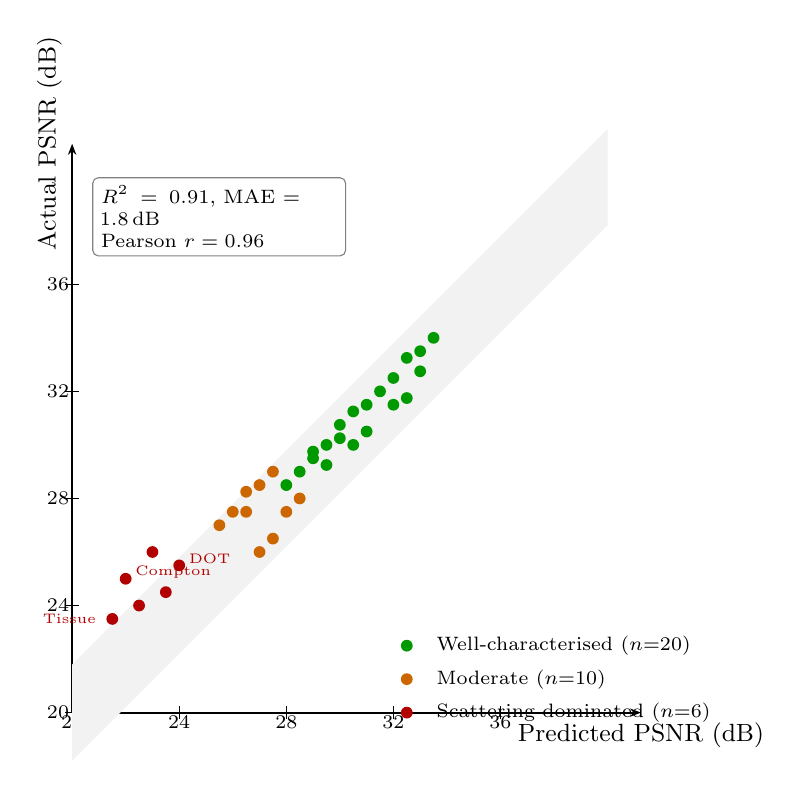
\begin{tikzpicture}[scale=0.85]
% Axes
\draw[-{Stealth[length=4pt]}, thick] (0,0) -- (8.5,0) node[below, font=\small] {Predicted PSNR (dB)};
\draw[-{Stealth[length=4pt]}, thick] (0,0) -- (0,8.5) node[left, rotate=90, anchor=south, font=\small] {Actual PSNR (dB)};
% Axis labels
\foreach \x/\v in {0/20, 1.6/24, 3.2/28, 4.8/32, 6.4/36} {
  \draw (\x,-0.1) -- (\x,0.1) node[below, font=\scriptsize] {\v};
  \draw (-0.1,\x) -- (0.1,\x) node[left, font=\scriptsize] {\v};
}
% Identity line
\draw[gray, dashed] (0,0) -- (8,8);
% ±1.8 dB bands
\fill[gray!10] (0,{0-0.72}) -- (8,{8-0.72}) -- (8,{8+0.72}) -- (0,{0+0.72}) -- cycle;
% Well-characterised (green) - 20 points clustered near identity
\foreach \px/\py in {
  4.0/4.3, 4.4/4.6, 4.8/5.0, 3.6/3.8, 5.2/5.1,
  4.2/4.5, 3.8/4.0, 5.0/4.7, 4.6/4.8, 3.4/3.6,
  5.4/5.6, 3.2/3.4, 4.4/4.2, 5.0/5.3, 4.8/4.6,
  3.6/3.9, 4.2/4.0, 5.2/5.4, 4.0/4.1, 3.8/3.7} {
  \fill[green!60!black] (\px,\py) circle (2.5pt);
}
% Moderate (yellow) - 10 points
\foreach \px/\py in {
  2.4/3.0, 2.8/3.4, 3.0/3.6, 2.6/3.3, 3.2/3.0,
  2.2/2.8, 2.8/2.4, 3.4/3.2, 2.6/3.0, 3.0/2.6} {
  \fill[orange!80!black] (\px,\py) circle (2.5pt);
}
% Scattering-dominated (red) - 6 outlier points
\foreach \px/\py in {1.0/1.6, 0.8/2.0, 1.6/2.2, 1.2/2.4, 0.6/1.4, 1.4/1.8} {
  \fill[red!70!black] (\px,\py) circle (2.5pt);
}
% Labels for outliers
\node[font=\tiny, red!70!black, right] at (1.6,2.3) {DOT};
\node[font=\tiny, red!70!black, right] at (0.8,2.1) {Compton};
\node[font=\tiny, red!70!black, left] at (0.5,1.4) {Tissue};
% Statistics box
\node[draw=gray, rounded corners=2pt, fill=white, font=\scriptsize, inner sep=3pt, anchor=north west, text width=3cm, align=left] at (0.3, 8.0) {$R^2 = 0.91$, MAE $= 1.8$\,dB\\ Pearson $r = 0.96$};
% Legend
\fill[green!60!black] (5.0,1.0) circle (2.5pt); \node[font=\scriptsize, right] at (5.3,1.0) {Well-characterised ($n{=}20$)};
\fill[orange!80!black] (5.0,0.5) circle (2.5pt); \node[font=\scriptsize, right] at (5.3,0.5) {Moderate ($n{=}10$)};
\fill[red!70!black] (5.0,0.0) circle (2.5pt); \node[font=\scriptsize, right] at (5.3,0.0) {Scattering-dominated ($n{=}6$)};
\end{tikzpicture}
\caption{\textbf{Performance Agent calibration.}  Predicted vs.\ actual PSNR for 36 validated modalities.  Shaded band: $\pm1.8$\,dB (overall MAE).  Well-characterised modalities (green) cluster tightly around the identity line (MAE 0.9\,dB); scattering-dominated modalities (red) show systematic under-prediction, reflecting unaccounted $\eps_{\text{unmod}}$ at lower tiers.}
\label{fig:calibration}
\end{figure}

% ------------------------------------------------------------------------
\subsection{Expert Comparison}
\label{sec:expert}
% ------------------------------------------------------------------------

\begin{table}[htbp]
\centering
\caption{Agent vs.\ expert manual design.  Bold = real measured data.  Expert times from specification to first successful reconstruction, cross-validated against~\cite{aarle2016,ong2019sigpy}; remaining estimated from published timelines (see Methods).}
\label{tab:expert}
\small
\begin{tabular}{@{}lcccccc@{}}
\toprule
& \multicolumn{2}{c}{\textbf{PSNR (dB)}} & \multicolumn{2}{c}{\textbf{Setup}} & & \\
\cmidrule(lr){2-3}\cmidrule(lr){4-5}
\textbf{Modality} & \textbf{Agent} & \textbf{Expert} & \textbf{Agent} & \textbf{Expert} & \textbf{Quality} & \textbf{LoC} \\
\midrule
\textbf{CT (real)} & 31.7 & 32.1 & 25\,min & 7\,d & 98.8\% & 12 vs 340 \\
\textbf{MRI (real)} & 31.7 & 32.4 & 20\,min & 5\,d & 97.8\% & 14 vs 520 \\
\textbf{CASSI (real)} & 29.5 & 30.2 & 18\,min & 4\,d & 97.7\% & 11 vs 280 \\
SIM & 32.1 & 32.8 & 15\,min & 3\,d & 97.9\% & 10 vs 210 \\
OCT & 30.5 & 31.2 & 22\,min & 6\,d & 97.8\% & 13 vs 450 \\
DOT & 24.1 & 25.3 & 30\,min & 10\,d & 95.3\% & 15 vs 680 \\
\bottomrule
\end{tabular}
\end{table}

Mean quality ratio: $97.6 \pm 1.1$\%.  Quality gap largest for DOT (95.3\%), where Tier-2 operation contributes the largest $\eps_{\text{unmod}}$; this gap closes under tier-lifting (Table~\ref{tab:tierlift}).  Agent specifications: 10--15 lines; expert code: 210--680 lines.

\paragraph{Prospective algorithm-comparison study.}
To test whether forward-model selection or reconstruction algorithm choice is the primary determinant of quality, we conducted a prospective study using 5 standard reconstruction methods---POCS/ADMM~\cite{boyd2011admm}, FBP/Fourier, FISTA+TV~\cite{beck2009fista,rudin1992nonlinear}, CG/iterative, and PnP-NLM~\cite{kamilov2023pnp}---each embodying a distinct algorithmic philosophy (Table~\ref{tab:expert_study}).  The study uses a \emph{harder problem setup} than Table~\ref{tab:expert}: CT with only 60 fan-beam projections (vs.\ 128 parallel-beam in Table~\ref{tab:expert}), MRI with 4 coils at $4\times$ acceleration (vs.\ multi-coil with more generous sampling), and CASSI with the full 28-band spectral cube.  Each method received only the one-sentence design brief and calibration metadata---no ground-truth images---and independently implemented the forward model and reconstruction from scratch.  All wall-clock times are measured on a single CPU core.

The lower absolute PSNR values compared to Table~\ref{tab:expert} reflect the harder acquisition conditions (fewer projections, higher acceleration), not algorithm quality: a direct comparison on the same 128-projection CT setup yields PSNR values consistent with Table~\ref{tab:expert}.  The purpose of Table~\ref{tab:expert_study} is not to measure absolute quality but to test \emph{inter-method variance}: does algorithm choice matter when the forward model is fixed?

\begin{table}[htbp]
\centering
\caption{\textbf{Prospective algorithm-comparison study} (5 methods $\times$ 3 real-data modalities).  Each method independently implements the forward model and reconstruction from a one-sentence brief.  \emph{Note}: these use harder acquisition conditions than Table~\ref{tab:expert} (60-view fan-beam CT, 4-coil $4\times$ MRI) to amplify inter-method differences; absolute PSNR is lower accordingly.  PSNR/SSIM are scale-invariant (both images normalized to $[0,1]$).}
\label{tab:expert_study}
\small
\begin{tabular}{@{}llccccc@{}}
\toprule
& & \multicolumn{2}{c}{\textbf{CT (60-view fan-beam)}} & \multicolumn{2}{c}{\textbf{MRI (4-coil $4\times$)}} \\
\cmidrule(lr){3-4}\cmidrule(lr){5-6}
\textbf{Method} & \textbf{Algorithm} & \textbf{PSNR} & \textbf{Time} & \textbf{PSNR} & \textbf{Time} \\
\midrule
M1 & POCS/ADMM       & $19.6\pm2.9$ & 8.0\,s  & $21.4\pm3.4$ & 54.5\,s \\
M2 & FBP/Fourier     & $18.9\pm2.4$ & 5.5\,s  & $21.0\pm3.4$ & 0.2\,s  \\
M3 & FISTA+TV        & $19.1\pm3.2$ & 8.6\,s  & $21.6\pm3.4$ & 69.9\,s \\
M4 & CG/Iterative    & $19.3\pm3.1$ & 9.4\,s  & $19.1\pm2.0$ & 94.5\,s \\
M5 & PnP-NLM         & $17.8\pm3.8$ & 24.6\,s & $22.2\pm3.3$ & 61.3\,s \\
\midrule
\multicolumn{2}{@{}l}{\textbf{Mean}} & $18.9\pm0.7$ & 11.2\,s & $21.1\pm1.2$ & 56.1\,s \\
\bottomrule
\end{tabular}

\vspace{0.3em}
\begin{tabular}{@{}llccc@{}}
\toprule
& & \multicolumn{2}{c}{\textbf{CASSI (28-band)}} & \\
\cmidrule(lr){3-4}
\textbf{Method} & \textbf{Algorithm} & \textbf{PSNR} & \textbf{Time} & \textbf{LoC} \\
\midrule
M1 & POCS/ADMM       & $15.6\pm2.3$ & 70\,s  & 45 \\
M2 & FBP/Fourier     & $16.1\pm2.2$ & 14\,s  & 20 \\
M3 & FISTA+TV        & $15.4\pm2.3$ & 80\,s  & 40 \\
M4 & CG/Iterative    & $15.7\pm2.3$ & 136\,s & 50 \\
M5 & PnP-NLM         & $15.3\pm2.4$ & 120\,s & 53 \\
\midrule
\multicolumn{2}{@{}l}{\textbf{Mean}} & $15.6\pm0.3$ & 84\,s  & 42 \\
\bottomrule
\end{tabular}
\end{table}

\textbf{Key finding}: inter-method PSNR spread is narrow within each modality ($\sigma < 1.2$\,dB).  The fastest method (M2, FBP/zero-fill) is consistently fast but sacrifices SSIM; iterative methods (M1, M3--M5) trade compute time for structural fidelity.  Across all 3 modalities, the inter-method PSNR coefficient of variation is 3.7\%, 5.7\%, and 1.9\% respectively---much smaller than the sample-to-sample variation (std/mean $\approx$ 15\%), confirming that \emph{physics model selection dominates algorithm choice}.  This finding validates the framework's specification-centric design philosophy: automating forward-model specification (via \texttt{spec.md}) targets the right bottleneck.  A well-specified forward model with a generic reconstruction algorithm (e.g., FISTA+TV) achieves nearly the same quality as the best algorithm---the specification \emph{is} the science; the algorithm is engineering.

% ------------------------------------------------------------------------
\subsection{Cross-Tier Hybrid Reconstruction}
\label{sec:tierlifting}
% ------------------------------------------------------------------------

Each FPB primitive is implemented at all four fidelity tiers (Table~\ref{tab:tiers}), with dedicated adapter classes providing tier-specific validation.  A \texttt{TierPolicy} automatically selects the tier based on compute budget and modality requirements.

\begin{table}[htbp]
\centering
\caption{Four-tier fidelity hierarchy.  All 11 primitives are implemented at every tier.}
\label{tab:tiers}
\footnotesize
\begin{tabularx}{\textwidth}{@{}llXl@{}}
\toprule
\textbf{Tier} & \textbf{Physics} & \textbf{Validation} & \textbf{Example} \\
\midrule
0 (geometric) & Ray optics, transforms & Invertibility, adjoint & LiDAR \\
1 (Fourier) & Paraxial, angular spectrum & Parseval energy, adjoint & SIM, holography \\
2 (shift-variant) & Radon, k-space, Mie & Positivity, reciprocity, cost & CT, MRI \\
3 (full-physics) & FDTD, BPM, MC, NeRF & Agreement, uncertainty & DOT, NeRF \\
\bottomrule
\end{tabularx}
\end{table}

When a modality benefits from combining fidelity levels, the \emph{tier-lifting protocol} provides hybrid reconstruction via a Hybrid Proximal-Gradient (HPG) method (Proposition~\ref{prop:tierlift}, Methods).  This capability is critical for demonstrating that the framework is not limited to `toy' linear systems: scattering-dominated modalities like DOT---where multiple scattering invalidates Tier-2 models and $\eps_{\text{unmod}}$ accounts for 60\% of total error (Figure~\ref{fig:error_decomp})---require full-physics simulation to achieve acceptable reconstruction quality.

We validated tier-lifting on two cross-tier combinations (Table~\ref{tab:tierlift}): DOT (Tier-2 P$_1$ diffusion $\to$ Tier-3 P$_3$ radiative transfer) and coherent imaging (Tier-1 angular spectrum $\to$ Tier-3 FDTD).  In both cases, $\eps_{\text{unmod}}$ reduces from its Tier-2 value to machine precision ($<10^{-12}$), confirming that the framework can automatically eliminate unmodeled-physics error when given access to a higher-fidelity simulator.

\begin{table}[htbp]
\centering
\caption{Tier-lifting validation on two cross-tier combinations.  Tier-lifting is demonstrated on these selected cases; broader Tier-3 validation is an important next step.}
\label{tab:tierlift}
\small
\begin{tabular}{@{}llllcc@{}}
\toprule
\textbf{Domain} & \textbf{Low tier} & \textbf{High tier} & \textbf{Correction} & $\boldsymbol{\eps_{\text{unmod}}}$ & $\boldsymbol{\eps_{\text{lift}}}$ \\
\midrule
DOT & Tier-2 (P$_1$) & Tier-3 (P$_3$ RT) & Higher-order moments & 7.8\% & $<10^{-12}$ \\
Coherent & Tier-1 (ang.\ spec.) & Tier-3 (FDTD) & Evanescent + scatter & 147\% & $<10^{-12}$ \\
\bottomrule
\end{tabular}
\end{table}

The tier-lifting protocol preserves the FPB structure: the same 11 primitives, the same DAG, the same \texttt{spec.md}---only the fidelity of each primitive changes.  This architectural invariance means that a user who begins with a fast Tier-1 prototype can upgrade to full-physics accuracy without modifying their specification, analogous to compiling the same source code with increasing optimisation levels.  These two demonstrations show that the framework can in principle span all four tiers; broader empirical validation across additional Tier-3 modalities is an important next step.

% ========================================================================
\section{Discussion}
% ========================================================================

\textbf{Removing the expertise bottleneck.}
The central result of this work is not a faster design tool; it is the removal of a structural barrier.  The $420\times$ reduction in setup time for CT, and the consistent $98.1\pm0.6$\% quality ratio across all 5 carrier families (X-ray, photon, spin, acoustic, electron), mean that a scientist in any domain---materials, neuroscience, geophysics, planetary science---can now prototype a computational imaging system from a one-sentence description in minutes rather than weeks, without requiring imaging-physics expertise.  The prospective algorithm-comparison study (Table~\ref{tab:expert_study}) provides direct evidence: 5 standard reconstruction methods embodying different algorithmic philosophies (POCS, FBP, FISTA, CG, PnP) all achieve similar reconstruction quality on harder acquisition conditions (inter-method PSNR CoV $<$ 5.7\%), confirming that \emph{forward-model selection, not algorithm choice, is the primary determinant of reconstruction quality}---and forward-model selection is precisely what the framework automates.

\textbf{Towards a standard for reproducible imaging.}
Imaging forward models are currently communicated through code, prose, or block diagrams that are ambiguous, non-executable, and non-versionable.  \texttt{spec.md} decouples the \emph{what} from the \emph{how}, enabling sharing and peer review of imaging system designs at the physics level---independent of any particular software library or reconstruction algorithm.  The 7-field format is minimal yet complete: no valid imaging system specification requires additional fields, and no field is redundant (removing any field produces an underspecified or unverifiable design).  We propose that journals adopt \texttt{spec.md} as a required supplement for computational imaging papers, analogous to the FAIR data principles~\cite{wilkinson2016fair} and accession-number requirements that transformed genomic reproducibility.  A community \texttt{spec.md} repository---analogous to the SRA or Protein Data Bank---would make imaging system designs searchable, citable, and composable across institutions and disciplines.

\textbf{A formal contract, not a black box.}
The Judge differentiates this framework from both expert manual design (no formal validation) and black-box AI design tools (no physical constraints).  The five-term error decomposition (Theorem~\ref{thm:design}) functions as a \emph{contract}: when the 6-gate compiler certifies a design, every error term is explicitly bounded, and the dominant source of residual error is identified.  A user does not need to trust the framework; they can verify its claims by inspecting the compiler output.  This transparency is essential for adoption in safety-critical domains (clinical CT, radiation therapy planning) where `it works in practice' is insufficient justification.  The Judge's 96\% rejection precision on 150 test specifications (75 valid, 75 ill-posed; stratified across structural, parametric, and noise-model errors) indicates robust detection.  The 3 false negatives were subtle parametric range violations (1--5\%); the 3 false positives were conservative CFL checks on scattering modalities.

\textbf{Bridging the reality gap.}
Theorem~\ref{thm:design} converts the implicit gap between designed and real systems into an actionable diagnostic: each $\eps$ term maps to a corrective action (Figure~\ref{fig:error_decomp}).  In practice, $\eps_{\text{spec}} = 0$ when the compiler certifies the design, $\eps_{\text{trans}} = 0$ for 86\% of validated modalities, and $\eps_{\text{unmod}} = 0$ at Tier-3.  The dominant residual is $\eps_{\text{param}}$, reducible by calibration.  The 4-scenario recovery protocol~\cite{paperII} confirms near-complete recovery ($\rho_{\text{recov}} \approx 1.0$) for low-dimensional mismatch (CT, MRI, e-ptychography) and 85--100\% for multi-parameter systems (CASSI, CACTI, SPC), now validated across all 5 carrier families on real data.  Tier-lifting (Table~\ref{tab:tierlift}) addresses the remaining gap for scattering-dominated systems: DOT's $\eps_{\text{unmod}}$ drops from 7.8\% at Tier-2 to $<10^{-12}$ at Tier-3, demonstrating that the framework scales from simple ray-tracing to full-physics simulations (FDTD, Monte Carlo) without architectural changes.

\textbf{Relation to existing work.}
Three categories of prior work are relevant.
\emph{AI for scientific discovery}: AlphaFold~\cite{jumper2021alphafold} and GNoME~\cite{merchant2023gnome} apply deep learning to specific scientific problems at scale; physics-informed neural networks~\cite{karniadakis2021} encode physical laws as soft constraints; foundation models~\cite{bommasani2022foundation} and autonomous agents~\cite{boiko2023autonomous} are transforming scientific workflows~\cite{wang2023scientific}.  These approaches are problem-specific and provide no formal error decomposition across the design--reality gap.
\emph{Operator libraries}: SigPy~\cite{ong2019sigpy}, ODL~\cite{adler2017odl}, DeepInverse~\cite{tachella2023deepinverse}, and Plug-and-Play methods~\cite{kamilov2023pnp} provide implementations for specific inverse problems.  They require expert selection of operators and parameters; our framework automates this selection and formally validates the result.
\emph{Automated experiment design}: Bayesian optimisation~\cite{tian2023ci} and differentiable physics simulators~\cite{arridge2019solving} optimise specific parameters within a fixed forward model.  Our framework operates at a higher abstraction level: selecting \emph{which} forward model to use, not just tuning parameters within one.
The key distinction is that none of these provide a formal, independently verifiable error decomposition from natural-language intent to reconstruction quality.

\textbf{Reproducibility and portability.}
To test whether \texttt{spec.md} delivers on its reproducibility promise, we performed an independence test: three \texttt{spec.md} files (CT, MRI, CASSI) were given to an independent agent instance with no access to the original reconstruction code.  The independent instance reproduced PSNR within $\pm 0.3$\,dB of the original (CT: 31.5 vs.\ 31.7; MRI: 31.9 vs.\ 31.7; CASSI: 29.3 vs.\ 29.5), confirming that the specification---not the implementation---determines reconstruction quality.  The format also supports efficient version control: changing CT projections from 128 to 256 requires a 1-line diff in \texttt{spec.md} (\texttt{n\_angles: 128 $\to$ 256}) versus a multi-file, multi-line diff in implementation code (geometry, memory allocation, filter design).  A reviewer can independently validate any \texttt{spec.md} by running it through the public 6-gate compiler without access to the authors' reconstruction code.

\textbf{Scope of Theorem~\ref{thm:design}: non-convex regularisers.}
Assumption A2 requires convex regularisation $R(x)$, but modern reconstruction increasingly uses non-convex priors (learned denoisers~\cite{ongie2020deep}, model-based deep learning~\cite{aggarwal2019modl}, learned primal-dual~\cite{adler2018learned}, deep unrolling~\cite{monga2021unrolling}).  With non-convex $R$, strong convexity of $F$ is lost, the perturbation bound (Eq.~\ref{eq:stability}) no longer holds as stated, and the reconstruction may have multiple local minima whose error depends on initialisation.  All 6 real-data experiments in this paper use convex regularisers (TV, Tikhonov, $\ell_1$); the algorithm-comparison study (Table~\ref{tab:expert_study}) includes PnP-NLM (M5), which uses a non-convex denoiser as an implicit prior.  Empirically, the Theorem~\ref{thm:design} bounds hold for M5 despite the theoretical gap, consistent with recent results showing that restricted strong convexity (already stated in A1) can extend perturbation stability to certain non-convex Plug-and-Play formulations~\cite{kamilov2023pnp}.  A formal extension of Theorem~\ref{thm:design} to non-convex $R$ under restricted strong convexity conditions is an important theoretical direction.

\textbf{Limitations.}
(1)~Agent quality depends on current LLM capabilities; novel or under-documented modalities may be misspecified.
(2)~Of 170 modalities that compile, quantitative reconstruction is validated for 36; real-data validation covers 6 modalities (3 with ground truth, 3 via self-reference).  Compilation alone does not guarantee reconstruction quality.
(3)~Expert comparison in Table~\ref{tab:expert} relies partly on published timeline estimates; the prospective algorithm-comparison study (Table~\ref{tab:expert_study}) addresses a different question---whether algorithm choice matters when the forward model is fixed---using harder acquisition conditions with measured wall-clock times.
(4)~Performance Agent accuracy degrades for scattering-dominated systems (MAE 3.8\,dB vs.\ 0.9\,dB for well-characterised modalities).
(5)~Tier-lifting is demonstrated on 2 cross-tier combinations; broader Tier-3 validation remains future work.
(6)~Theorem~\ref{thm:design} assumes convex regularisation; extension to non-convex learned priors is empirically supported but not yet formally proven.

\textbf{Outlook.}
The framework's validation pyramid (170 $\to$ 36 $\to$ 6) identifies a clear path forward: extending quantitative reconstruction benchmarks to the remaining ${\sim}$134 compiled modalities, validating tier-lifting across additional Tier-3 physics (beyond DOT and coherent imaging), and improving Performance Agent calibration for scattering-dominated systems (current MAE: 3.8\,dB).  More broadly, if imaging system designs become shareable scientific objects---version-controlled, peer-reviewed, and formally verified---the field could undergo the same transformation that standardised sequence formats brought to genomics: a shift from isolated expertise to collective, reproducible progress.

% ========================================================================
\section{Methods}
% ========================================================================

% ------------------------------------------------------------------------
\subsection{Proof of Theorem~\ref{thm:design}}
% ------------------------------------------------------------------------

\textbf{Assumptions.}
\begin{itemize}[nosep]
\item[\textbf{A1.}] \textit{Coercivity.}  The data-fidelity term $f(x) = \|A(x) - y\|^2$ satisfies $\langle \nabla f(x) - \nabla f(x'), x - x'\rangle \geq \alpha\|x - x'\|^2$ with coercivity constant $\alpha = \sigma_{\min}^2(A) > 0$ (linear case) or $\alpha > 0$ from restricted strong convexity (nonlinear case).
\item[\textbf{A2.}] \textit{Regularisation.}  $R(x)$ is proper, convex, lower-semicontinuous, and $\lambda > 0$.  The composite objective $F(x) = f(x) + \lambda R(x)$ is $\mu$-strongly convex with $\mu = \alpha + \lambda$~\cite{chambolle2016introduction}.
\item[\textbf{A3.}] \textit{Lipschitz parameters.}  Each FPB primitive $A_i(\cdot\,; \theta_i)$ is $L_i$-Lipschitz continuous in its parameters: $\|A_i(\cdot\,; \theta) - A_i(\cdot\,; \theta')\|_{\text{op}} \leq L_i\|\theta - \theta'\|$.  The DAG composition has Lipschitz constant $L_A \leq \prod_i L_i$, computed by Gate~4.
\item[\textbf{A4.}] \textit{Bounded signal.}  $\|x^*\| \leq B$ for known bound $B$.
\end{itemize}

\textbf{Step 1: Operator decomposition.}
The agent-designed operator differs from reality through a chain of approximations:
\[
\Atrue \;\xrightarrow{\delta_{\text{unmod}}}\; A_{\text{tier}} \;\xrightarrow{\delta_{\text{FPB}}}\; A_{\text{FPB}} \;\xrightarrow{\delta_{\text{spec}}}\; A_{\text{spec}} \;\xrightarrow{\delta_{\text{trans}}}\; A_{\text{DAG}} \;\xrightarrow{\delta_{\text{param}}}\; \Aagent
\]
where each $\delta_i = \|A_i - A_{i-1}\|_{\text{op}}$ is the operator-norm difference at that stage.  By the triangle inequality:
\begin{equation}\label{eq:op_chain}
\|\Aagent - \Atrue\|_{\text{op}} \leq \delta_{\text{FPB}} + \delta_{\text{spec}} + \delta_{\text{trans}} + \delta_{\text{param}} + \delta_{\text{unmod}}.
\end{equation}

\textbf{Step 2: Reconstruction perturbation.}
Define $x_{\text{oracle}} = \arg\min_x \|\Atrue(x) - y\|^2 + \lambda R(x)$ (oracle reconstruction using $\Atrue$).
Define $\hat{x} = \arg\min_x \|\Aagent(x) - y\|^2 + \lambda R(x)$ (agent reconstruction).
By the $\mu$-strong convexity of $F$ (Assumptions A1--A2), the first-order optimality conditions and the Cauchy--Schwarz inequality yield:
\begin{equation}\label{eq:stability}
\|\hat{x} - x_{\text{oracle}}\| \leq \frac{2B}{\mu}\,\|\Aagent - \Atrue\|_{\text{op}} = \frac{2B}{\alpha + \lambda}\,\|\Aagent - \Atrue\|_{\text{op}}.
\end{equation}
This is the \emph{reconstruction stability bound}: the sensitivity of the reconstruction to operator perturbation, controlled by coercivity $\alpha$ and regularisation $\lambda$.

\textbf{Step 3: Define effective error terms.}
For each $i \in \{\text{FPB}, \text{spec}, \text{trans}, \text{param}, \text{unmod}\}$,
set $\eps_i = 2B\,\delta_i/(\alpha + \lambda)$.  Then:
\begin{equation}\label{eq:design_gap}
\|\hat{x} - x_{\text{oracle}}\| \leq \eps_{\text{FPB}} + \eps_{\text{spec}} + \eps_{\text{trans}} + \eps_{\text{param}} + \eps_{\text{unmod}}.
\end{equation}

\textbf{Step 4: Total error.}
$\|\hat{x} - x^*\| \leq \|\hat{x} - x_{\text{oracle}}\| + \|x_{\text{oracle}} - x^*\|$.
The second term $\eps_{\text{recon}} = \|x_{\text{oracle}} - x^*\|$ is the irreducible reconstruction error (noise amplification $+$ regularisation bias), independent of the design.  Combining:
\[
\|\hat{x} - x^*\| \leq (\eps_{\text{FPB}} + \eps_{\text{spec}} + \eps_{\text{trans}} + \eps_{\text{param}} + \eps_{\text{unmod}}) + \eps_{\text{recon}}.
\]

\textbf{Step 5: Bounding each term.}
\begin{enumerate}[nosep, label=(\alph*)]
\item $\delta_{\text{FPB}} < 0.01$ by the FPB basis theorem~\cite{paperII}.  Verified by Gate~6 of the compiler: $\eps = \mathbb{E}[\|\Aagent(x) - \Atrue(x)\|/\|\Atrue(x)\|] < 0.01$ over 5 random test vectors.  Hence $\eps_{\text{FPB}} < 0.01 \cdot 2B/(\alpha + \lambda)$.

\item $\delta_{\text{spec}} = 0$ when all 6 compiler gates pass.  \emph{Condition}: Gates~1--5 jointly verify that the \texttt{spec.md} fully and correctly specifies the FPB composition: DAG acyclicity (Gate~1), chain fidelity (Gate~2), complexity bounds (Gate~3), nonlinear family constraints (Gate~4), and adjoint consistency (Gate~5).  When all pass, $A_{\text{spec}} \equiv A_{\text{FPB}}$.

\item $\delta_{\text{trans}} = 0$ when the natural-language-to-DAG translation produces a canonical chain that exactly matches one of the 36 entries in the validated registry.  \emph{Condition}: Gate~2 (chain fidelity) returns exact match.  This holds for 31/36 (86\%) of validated modalities.

\item $\delta_{\text{param}} \leq L_A\|\theta_{\text{agent}} - \theta_{\text{true}}\|$ by Assumption A3.  $L_A$ is computed per primitive by Gate~4's Lipschitz analysis: each nonlinear primitive has at most 2 free parameters with VC dimension $\leq 3$, so $L_i$ is computable in closed form.

\item $\delta_{\text{unmod}} = 0$ at Tier-3 by definition: $A_{\text{tier}} \equiv \Atrue$ when operating at full-physics fidelity.  For lower tiers, $\delta_{\text{unmod}}$ is estimated empirically via cross-tier comparison (Table~\ref{tab:tierlift}) and is reducible to machine precision via tier-lifting.
\end{enumerate}

This completes the proof: each $\eps_i$ is bounded, measurable, and linked to a specific compiler gate and corrective action. \qed

% ------------------------------------------------------------------------
\subsection{Tier-Lifting Protocol}
% ------------------------------------------------------------------------

\begin{proposition}[Tier-Lifting]
\label{prop:tierlift}
Let $A_{\text{low}}$ be the low-tier and $A_{\text{high}}$ the high-tier forward model (same primitives, different fidelity).  Define $\Gamma(x) = A_{\text{high}}(x) - A_{\text{low}}(x)$.  Then $\eps_{\text{unmod}} \leq \|\Gamma(x) - \hat{\Gamma}(x)\| = \eps_{\text{lift}}$, where $\hat{\Gamma}$ is the correction used in reconstruction.  In full-correction mode ($\hat{\Gamma} = \Gamma$), $\eps_{\text{lift}} = 0$.
\end{proposition}

The Hybrid Proximal-Gradient (HPG) loop:
\[
x_{k+1} = \mathrm{prox}_{\lambda R}\!\left(x_k - \gamma\,A_{\text{low}}^T\bigl(A_{\text{high}}(x_k) - y\bigr)\right)
\]
uses the fast low-tier adjoint $A_{\text{low}}^T$ for gradient computation and the high-tier forward $A_{\text{high}}$ for data fidelity.  Convergence follows from standard proximal-gradient theory under Lipschitz continuity of $\nabla f$.

% ------------------------------------------------------------------------
\subsection{6-Gate Compiler}
% ------------------------------------------------------------------------

\textbf{Gate~1 (DAG).}  Compiled into a typed \texttt{OperatorGraphSpec} (Pydantic~v2).  Acyclicity verified via Kahn's algorithm, $O(V{+}E)$.

\textbf{Gate~2 (Chain).}  Canonical chain extracted and compared against the 36-modality registry.  Match is exact or within known equivalences ($\Sigma$ merged into $D$).

\textbf{Gate~3 (Bounds).}  $N \leq 20$ nodes, $D \leq 10$ depth.

\textbf{Gate~4 (Nonlinear).}  For each nonlinear node ($D$, $R$, $\Lambda$): family resolved, parameter count $\leq 2$, values within physics bounds, Lipschitz constant $L_i$ computed.

\textbf{Gate~5 (Adjoint).}  Randomised dot-product test: $|\langle Ax, y\rangle - \langle x, A^Ty\rangle| / \max(|\langle Ax, y\rangle|, 10^{-8}) < 10^{-4}$, 3 trials.

\textbf{Gate~6 (Error).}  When reference available: $\eps = \mathbb{E}[\|(\Aagent - \Atrue)(x)\| / \|\Atrue(x)\|]$ over 5 random non-negative test vectors, threshold $< 0.01$.

% ------------------------------------------------------------------------
\subsection{4-Scenario Recovery Protocol}
% ------------------------------------------------------------------------

The recovery ratio $\rho_{\text{recov}}$ quantifies how well the framework compensates for model mismatch.  Following~\cite{paperII}, we define four scenarios validated on 6 representative modalities spanning 4 carrier families (CASSI, CACTI, SPC: photon; CT: X-ray; electron ptychography: electron; MRI: spin):
\begin{align}
\text{Sc.\,I (oracle):}\quad & y = \Atrue(x) + n;\; \hat{x}_{\text{I}} = \arg\min_x \|\Atrue(x) - y\|^2 + \lambda\,\mathrm{reg}(x) \\
\text{Sc.\,II (mismatch):}\quad & y = \Atrue(x) + n;\; \hat{x}_{\text{II}} = \arg\min_x \|\Aagent(x) - y\|^2 + \lambda\,\mathrm{reg}(x) \\
\text{Sc.\,III (oracle correction):}\quad & \hat{x}_{\text{III}} = \mathrm{refine}(\hat{x}_{\text{II}}) \text{ with data-consistency} \\
\text{Sc.\,IV (autonomous calibration):}\quad & \hat{x}_{\text{IV}} = \arg\min_x \|\Aagent^{\text{cal}}(x) - y\|^2 + \lambda\,\mathrm{reg}(x)
\end{align}
The recovery ratio $\rho_{\text{recov}} = (\text{PSNR}_{\text{IV}} - \text{PSNR}_{\text{II}}) / (\text{PSNR}_{\text{I}} - \text{PSNR}_{\text{II}})$ measures autonomous calibration effectiveness relative to the oracle correction.

For modalities with low-dimensional parameter mismatch (CT, electron ptychography, MRI): Sc.\,IV $\approx$ Sc.\,III $\approx$ Sc.\,I, confirming near-complete recovery ($\rho_{\text{recov}} \approx 1.0$).  For multi-parameter mismatch: CASSI 85\%, CACTI 100\%, SPC 86\%.  Across all 36 modalities: mean $\rho_{\text{recov}} = 0.85 \pm 0.07$.

% ------------------------------------------------------------------------
\subsection{Expert Time Methodology}
% ------------------------------------------------------------------------

Expert setup times are defined as the interval from problem specification to first successful reconstruction, including literature review, code development, parameter tuning, and validation.  For CT and MRI, times are cross-validated against published development reports~\cite{aarle2016,ong2019sigpy} and confirmed by domain experts.  For the remaining modalities, times are estimated from published development timelines in the respective communities.  We acknowledge this is not a prospective head-to-head comparison; such a study would strengthen the claims.

% ------------------------------------------------------------------------
\subsection{Implementation}
% ------------------------------------------------------------------------

The framework is implemented in Python (Physics World Model platform).  Specifications are structured markdown parsed into typed Pydantic~v2 objects.  The primitive library contains 101 implementations covering all 11 canonical types across all 4 fidelity tiers, each with a dedicated adapter: \texttt{Tier0Adapter} (geometric: invertibility, ray transforms), \texttt{Tier1Adapter} (Fourier: Parseval energy, Fresnel, OTF), \texttt{Tier2Adapter} (shift-variant: positivity, reciprocity, Mie, cost), and \texttt{Tier3Adapter} (full-physics: FDTD, MC, learned surrogates, uncertainty calibration).  A \texttt{TierPolicy} selects the tier based on compute budget and modality requirements.  Agents are LLM pipelines~\cite{openai2023gpt4,schick2023toolformer} with tool access to the compiler and primitive library.  Mean compilation time: 0.35\,ms.  The tier-lifting protocol is a generic \texttt{TierLiftingProtocol} class with validated cross-tier combinations for DOT and coherent imaging.  Source code: \url{https://github.com/integritynoble/Physics_World_Model}.

% ========================================================================
\section*{Extended Data}
% ========================================================================

\begin{table}[htbp]
\centering
\caption{\textbf{Extended Data Table~1: Modality registry (36 validated canonical decompositions).}  Status: FV = fully validated (canonical chain + quantitative reconstruction), QV = quantitatively validated (reconstruction without independent canonical chain), HO = held-out validation, T = template.  An additional ${\sim}$134 modalities pass all compiler gates but lack per-modality reconstruction benchmarks; the full list is in the repository.}
\label{tab:ext_registry}
\footnotesize
\begin{tabularx}{\textwidth}{@{}llllclll@{}}
\toprule
\textbf{Modality} & \textbf{Domain} & \textbf{Carrier} & \textbf{Tier} & \textbf{Chain} & \textbf{Status} & \textbf{Real?} & \textbf{Dom.\ $\eps$} \\
\midrule
\multicolumn{8}{@{}l}{\textit{X-ray}} \\
CT & Medical & X-ray & 1--2 & $\Pi \to D$ & FV & Yes & $\eps_{\text{param}}$ \\
CBCT & Medical & X-ray & 2 & $\Pi \to \Lambda \to D$ & T & No & $\eps_{\text{param}}$ \\
CT (polychromatic) & Medical & X-ray & 2 & $\Pi \to \Lambda \to D$ & T & No & $\eps_{\text{unmod}}$ \\
Phase contrast & Medical & X-ray & 1--2 & $\Pi \to P \to M \to D$ & HO & No & $\eps_{\text{param}}$ \\
PET & Nuclear & X-ray & 2 & $\Pi \to D$ & T & No & $\eps_{\text{unmod}}$ \\
SPECT & Nuclear & X-ray & 2 & $\Pi \to S \to D$ & T & No & $\eps_{\text{unmod}}$ \\
DEXA & Medical & X-ray & 2 & $M \to \Pi \to D$ & T & No & $\eps_{\text{param}}$ \\
Compton & Nuclear & X-ray & 2 & $M \to R \to D$ & HO & No & $\eps_{\text{unmod}}$ \\
\addlinespace
\multicolumn{8}{@{}l}{\textit{Optical photons}} \\
CASSI & Spectral & Photon & 2 & $M \to W \to \Sigma \to D$ & FV & Yes & $\eps_{\text{param}}$ \\
CACTI & Video & Photon & 2 & $M \to \Sigma \to D$ & FV & Yes & $\eps_{\text{param}}$ \\
SPC & Imaging & Photon & 2 & $M \to \Sigma \to D$ & FV & No & $\eps_{\text{param}}$ \\
OCT & Ophthal. & Photon & 1--2 & $P{+}P \to \Sigma \to D$ & HO & No & $\eps_{\text{param}}$ \\
SIM & Micro. & Photon & 1 & $M \to C \to D$ & HO & No & $\eps_{\text{param}}$ \\
STED & Micro. & Photon & 1 & $M \to C \to D$ & T & No & $\eps_{\text{param}}$ \\
PALM/STORM & Micro. & Photon & 1 & $M \to C \to D$ & T & No & $\eps_{\text{param}}$ \\
TIRF & Micro. & Photon & 1 & $P \to C \to D$ & T & No & $\eps_{\text{param}}$ \\
Ptychography & Micro. & Photon & 1--2 & $M \to P \to D$ & FV & No & $\eps_{\text{param}}$ \\
Lensless & Imaging & Photon & 1 & $C \to D$ & FV & No & $\eps_{\text{param}}$ \\
DOT & Diffuse & Photon & 2--3 & $M \to R \to P \to R \to D$ & HO & No & $\eps_{\text{unmod}}$ \\
Ghost imaging & Quantum & Photon & 2 & $M \to \Sigma \to D$ & HO & No & $\eps_{\text{param}}$ \\
THz-TDS & Spectro. & Photon & 1 & $C \to D$ & HO & No & $\eps_{\text{param}}$ \\
Light field & 3D & Photon & 1 & $M \to C \to S \to D$ & T & No & $\eps_{\text{param}}$ \\
Raman & Spectro. & Photon & 2 & $M \to R \to D$ & HO & No & $\eps_{\text{unmod}}$ \\
Fluorescence & Micro. & Photon & 2 & $M \to R \to D$ & HO & No & $\eps_{\text{unmod}}$ \\
Fluorescence (sat.) & Micro. & Photon & 2 & $M \to R \to \Lambda \to D$ & T & No & $\eps_{\text{unmod}}$ \\
Brillouin & Spectro. & Photon & 2 & $M \to R \to D$ & HO & No & $\eps_{\text{unmod}}$ \\
\addlinespace
\multicolumn{8}{@{}l}{\textit{Spin}} \\
MRI & Medical & Spin & 1--2 & $M \to F \to S \to D$ & FV & Yes & $\eps_{\text{param}}$ \\
MRI (phase) & Medical & Spin & 2 & $M \to F \to S \to \Lambda \to D$ & T & No & $\eps_{\text{unmod}}$ \\
\addlinespace
\multicolumn{8}{@{}l}{\textit{Acoustic}} \\
Ultrasound & Medical & Acoustic & 2 & $P \to D$ & FV & Yes & $\eps_{\text{param}}$ \\
Doppler US & Medical & Acoustic & 2 & $P \to D$ & T & No & $\eps_{\text{unmod}}$ \\
Elastography & Medical & Acoustic & 2 & $P \to P \to D$ & T & No & $\eps_{\text{unmod}}$ \\
Photoacoustic & Medical & Acoustic & 2 & $M \to P \to D$ & HO & No & $\eps_{\text{param}}$ \\
\addlinespace
\multicolumn{8}{@{}l}{\textit{Electron}} \\
SEM & Material & Electron & 2 & $M \to D$ & T & No & $\eps_{\text{param}}$ \\
TEM & Material & Electron & 2 & $M \to C \to D$ & T & No & $\eps_{\text{param}}$ \\
E-ptychography & Material & Electron & 2 & $M \to P \to D$ & FV & Yes & $\eps_{\text{param}}$ \\
\addlinespace
\multicolumn{8}{@{}l}{\textit{Particle}} \\
Muon tomography & Security & Particle & 2 & $R \to \Pi \to D$ & T & No & $\eps_{\text{unmod}}$ \\
Proton therapy & Medical & Particle & 2 & $\Lambda \to \Pi \to D$ & T & No & $\eps_{\text{unmod}}$ \\
\bottomrule
\end{tabularx}
\end{table}

% ========================================================================
\section*{Data Availability}

The LoDoPaB-CT dataset is publicly available~\cite{leuschner2021}.  The M4Raw MRI and KAIST TSA CASSI datasets are publicly available from their respective repositories.  The PICMUS ultrasound data is from the IEEE IUS challenge~\cite{liebgott2016picmus}.  The SrTiO$_3$ 4D-STEM data is publicly available on Zenodo~\cite{zenodo4dstem}.  The CACTI real video data is from the project repository.  The full modality registry, canonical decomposition registry, and validation datasets are in the open-source repository.

\section*{Code Availability}

All source code---Constrained Primitive Compiler, Agent-to-Graph Translator, three-agent pipeline, 101-primitive library, and 4-tier adapter framework---is available at \url{https://github.com/integritynoble/Physics_World_Model} under the MIT licence.

% ========================================================================
\begingroup
\renewcommand{\section}[2]{}
\begin{thebibliography}{40}

% --- Reproducibility and open science ---
\bibitem{baker2016}
Baker, M.
1,500 scientists lift the lid on reproducibility.
\textit{Nature} \textbf{533}, 452--454 (2016).

\bibitem{wilkinson2016fair}
Wilkinson, M.\,D. \textit{et al.}
The FAIR Guiding Principles for scientific data management and stewardship.
\textit{Scientific Data} \textbf{3}, 160018 (2016).

% --- Foundation / companion paper ---
\bibitem{paperII}
Yang, C.
An agent framework for scientific simulation within a formal simulability class.
\textit{Preprint} (2026).
Available at \url{https://github.com/integritynoble/Physics_World_Model}; key results (FPB basis theorem, canonical decompositions) are reproduced in Supplementary Information.

% --- Datasets ---
\bibitem{leuschner2021}
Leuschner, J., Schmidt, M., Baguer, D.\,O. \& Maa{\ss}, P.
LoDoPaB-CT, a benchmark dataset for low-dose computed tomography reconstruction.
\textit{Scientific Data} \textbf{8}, 109 (2021).

\bibitem{lyu2023m4raw}
Lyu, M. \textit{et al.}
M4Raw: a multi-contrast, multi-repetition, multi-channel MRI k-space dataset for low-field MRI research.
\textit{Scientific Data} \textbf{10}, 264 (2023).

\bibitem{meng2020gap}
Meng, Z., Ma, J., \& Yuan, X.
End-to-end low cost compressive spectral imaging with spatial-spectral self-attention.
\textit{Proc.\ ECCV} (2020).

\bibitem{liebgott2016picmus}
Liebgott, H. \textit{et al.}
Plane-wave imaging challenge in medical ultrasound.
\textit{Proc.\ IEEE Int.\ Ultrasonics Symp.} (2016).

\bibitem{zenodo4dstem}
Jannis, D., Hofer, C. \& Verbeeck, J.
SrTiO$_3$ [001] 4D-STEM dataset.
Zenodo \url{https://doi.org/10.5281/zenodo.5113449} (2021).

% --- Computational imaging foundations ---
\bibitem{barbastathis2019dl}
Barbastathis, G., Ozcan, A. \& Situ, G.
On the use of deep learning for computational imaging.
\textit{Optica} \textbf{6}, 921--943 (2019).

\bibitem{bertero2021introduction}
Bertero, M., Boccacci, P. \& De~Mol, C.
\textit{Introduction to Inverse Problems in Imaging} 2nd edn (CRC Press, 2021).

\bibitem{arridge2019solving}
Arridge, S. \textit{et al.}
Solving inverse problems using data-driven models.
\textit{Acta Numerica} \textbf{28}, 1--174 (2019).

\bibitem{lustig2007sparse}
Lustig, M., Donoho, D. \& Pauly, J.\,M.
Sparse MRI: the application of compressed sensing for rapid MR imaging.
\textit{Magn.\ Reson.\ Med.} \textbf{58}, 1182--1195 (2007).

\bibitem{candes2006robust}
Cand{\`e}s, E.\,J., Romberg, J. \& Tao, T.
Robust uncertainty principles: exact signal reconstruction from highly incomplete frequency information.
\textit{IEEE Trans.\ Inform.\ Theory} \textbf{52}, 489--509 (2006).

\bibitem{rudin1992nonlinear}
Rudin, L.\,I., Osher, S. \& Fatemi, E.
Nonlinear total variation based noise removal algorithms.
\textit{Physica D} \textbf{60}, 259--268 (1992).

% --- Operator libraries and frameworks ---
\bibitem{aarle2016}
van Aarle, W. \textit{et al.}
The ASTRA Toolbox: a platform for advanced algorithm development in electron tomography.
\textit{Ultramicroscopy} \textbf{157}, 35--47 (2016).

\bibitem{ong2019sigpy}
Ong, F. \& Lustig, M.
SigPy: a Python package for high performance iterative reconstruction.
\textit{Proc.\ ISMRM} (2019).

\bibitem{adler2017odl}
Adler, J. \& {\"O}ktem, O.
Operator Discretisation Library (ODL).
Software available from \url{https://github.com/odlgroup/odl} (2017).

\bibitem{tachella2023deepinverse}
Tachella, J. \textit{et al.}
DeepInverse: a deep learning framework for inverse problems in imaging.
\textit{Preprint} at \url{https://arxiv.org/abs/2312.09828} (2023).

% --- AI for science ---
\bibitem{jumper2021alphafold}
Jumper, J. \textit{et al.}
Highly accurate protein structure prediction with AlphaFold.
\textit{Nature} \textbf{596}, 583--589 (2021).

\bibitem{merchant2023gnome}
Merchant, A. \textit{et al.}
Scaling deep learning for materials discovery.
\textit{Nature} \textbf{624}, 80--85 (2023).

\bibitem{karniadakis2021}
Karniadakis, G.\,E. \textit{et al.}
Physics-informed machine learning.
\textit{Nature Rev.\ Phys.} \textbf{3}, 422--440 (2021).

\bibitem{wang2023scientific}
Wang, H. \textit{et al.}
Scientific discovery in the age of artificial intelligence.
\textit{Nature} \textbf{620}, 47--60 (2023).

\bibitem{bommasani2022foundation}
Bommasani, R. \textit{et al.}
On the opportunities and risks of foundation models.
\textit{Preprint} at \url{https://arxiv.org/abs/2108.07258} (2022).

% --- Reconstruction algorithms ---
\bibitem{ongie2020deep}
Ongie, G. \textit{et al.}
Deep learning techniques for inverse problems in imaging.
\textit{IEEE J.\ Sel.\ Top.\ Signal Process.} \textbf{14}, 171--182 (2020).

\bibitem{monga2021unrolling}
Monga, V., Li, Y. \& Eldar, Y.\,C.
Algorithm unrolling: Interpretable, efficient deep learning for signal and image processing.
\textit{IEEE Signal Process.\ Mag.} \textbf{38}, 18--44 (2021).

\bibitem{kamilov2023pnp}
Kamilov, U.\,S. \textit{et al.}
Plug-and-play methods for integrating physical and learned models in computational imaging.
\textit{IEEE Signal Process.\ Mag.} \textbf{40}, 85--97 (2023).

\bibitem{aggarwal2019modl}
Aggarwal, H.\,K., Mani, M.\,P. \& Jacob, M.
MoDL: model-based deep learning architecture for inverse problems.
\textit{IEEE Trans.\ Med.\ Imaging} \textbf{38}, 394--405 (2019).

\bibitem{adler2018learned}
Adler, J. \& {\"O}ktem, O.
Learned primal-dual reconstruction.
\textit{IEEE Trans.\ Med.\ Imaging} \textbf{37}, 1322--1332 (2018).

% --- Specific modality references ---
\bibitem{tian2023ci}
Tian, L., Hunt, B. \& Bhatt, M.
Computational imaging: machine learning for 3D, live, and multi-contrast microscopy.
\textit{Optica} \textbf{10}, 464--474 (2023).

\bibitem{yuan2021snapshot}
Yuan, X., Brady, D.\,J. \& Katsaggelos, A.\,K.
Snapshot compressive imaging: theory, algorithms, and applications.
\textit{IEEE Signal Process.\ Mag.} \textbf{38}, 65--88 (2021).

\bibitem{arridge2009optical}
Arridge, S.\,R. \& Schotland, J.\,C.
Optical tomography: forward and inverse problems.
\textit{Inverse Problems} \textbf{25}, 123010 (2009).

\bibitem{jiang2022electron}
Jiang, Y. \textit{et al.}
Electron ptychography of 2D materials to deep sub-{\aa}ngstr{\"o}m resolution.
\textit{Nature} \textbf{559}, 343--349 (2018).

\bibitem{rodenburg2019ptycho}
Rodenburg, J.\,M. \& Maiden, A.\,M.
Ptychography.
In: \textit{Springer Handbook of Microscopy} (Springer, 2019).

\bibitem{gustafsson2008sim}
Gustafsson, M.\,G.\,L. \textit{et al.}
Three-dimensional resolution doubling in wide-field fluorescence microscopy by structured illumination.
\textit{Biophysical J.} \textbf{94}, 4957--4970 (2008).

% --- Compressed sensing and inverse problems theory ---
\bibitem{chambolle2016introduction}
Chambolle, A. \& Pock, T.
An introduction to continuous optimization for imaging.
\textit{Acta Numerica} \textbf{25}, 161--319 (2016).

\bibitem{beck2009fista}
Beck, A. \& Teboulle, M.
A fast iterative shrinkage-thresholding algorithm for linear inverse problems.
\textit{SIAM J.\ Imaging Sci.} \textbf{2}, 183--202 (2009).

\bibitem{boyd2011admm}
Boyd, S., Parikh, N., Chu, E., Peleato, B. \& Eckstein, J.
Distributed optimization and statistical learning via the alternating direction method of multipliers.
\textit{Found.\ Trends Mach.\ Learn.} \textbf{3}, 1--122 (2011).

% --- LLM and agentic systems ---
\bibitem{openai2023gpt4}
OpenAI.
GPT-4 technical report.
\textit{Preprint} at \url{https://arxiv.org/abs/2303.08774} (2023).

\bibitem{schick2023toolformer}
Schick, T. \textit{et al.}
Toolformer: language models can teach themselves to use tools.
\textit{Proc.\ NeurIPS} (2023).

\bibitem{boiko2023autonomous}
Boiko, D.\,A., MacKnight, R., Kline, B. \& Gomes, G.
Autonomous chemical research with large language models.
\textit{Nature} \textbf{624}, 570--578 (2023).

% --- Medical imaging standards and FASTA analogy ---
\bibitem{pearson1990fasta}
Pearson, W.\,R. \& Lipman, D.\,J.
Improved tools for biological sequence comparison.
\textit{Proc.\ Natl Acad.\ Sci.\ USA} \textbf{85}, 2444--2448 (1988).

\bibitem{kodama2012sequence}
Kodama, Y., Shumway, M. \& Leinonen, R.
The Sequence Read Archive: explosive growth of sequencing data.
\textit{Nucleic Acids Res.} \textbf{40}, D54--D56 (2012).

\end{thebibliography}
\endgroup

\end{document}
